% ===========================================================================
%  Rapport de conduite de projet Data & ML — OC_P13
%  Mise en production du modèle de prédiction énergétique de Seattle
%
%  Sur Overleaf : déposer ce dossier tel quel, choisir main.tex comme document
%  principal, compilateur pdfLaTeX. Aucun paquet à installer.
% ===========================================================================

\documentclass[11pt,a4paper]{article}

% ===========================================================================
%  Préambule — rapport de conduite de projet OC_P13
%
%  Compilation : pdfLaTeX (le compilateur par défaut d'Overleaf).
%  Tous les paquets utilisés sont dans la distribution TeX Live standard,
%  donc rien à installer.
% ===========================================================================

\usepackage[T1]{fontenc}
\usepackage[utf8]{inputenc}
\usepackage[french]{babel}
\usepackage{newtxtext,newtxmath}
\usepackage{microtype}

\usepackage[a4paper,margin=2.4cm,headheight=15pt]{geometry}
\usepackage{graphicx}
\usepackage{booktabs}
\usepackage{tabularx}
\usepackage{array}
\usepackage{longtable}
\usepackage{xcolor}
\usepackage{enumitem}
\usepackage{fancyhdr}
\usepackage{caption}
\usepackage{float}
\usepackage{csquotes}

% Nombres : separateur de milliers par espace fine, virgule decimale.
\usepackage{siunitx}
\sisetup{
  group-separator = {\,},
  group-minimum-digits = 4,
  output-decimal-marker = {,},
  detect-all,
}

\usepackage[hidelinks]{hyperref}
\hypersetup{
  pdftitle={Mise en production d'un modèle de prédiction énergétique},
  pdfauthor={Kevin Lebayle},
  colorlinks=true,
  linkcolor=accent,
  urlcolor=accent,
  citecolor=accent,
}

% --- Couleurs -------------------------------------------------------------
% Les deux cibles du modèle gardent dans le rapport les couleurs qu'elles ont
% dans l'application : bleu pour l'énergie, orange pour les émissions.
\definecolor{accent}{HTML}{2A78D6}
\definecolor{emissions}{HTML}{EB6834}
\definecolor{encadre}{HTML}{F4F6F8}
\definecolor{filet}{HTML}{D5DBE1}
\definecolor{gristexte}{HTML}{52514E}

% --- En-têtes -------------------------------------------------------------
\pagestyle{fancy}
\fancyhf{}
\renewcommand{\headrulewidth}{0.4pt}
\fancyhead[L]{\small\color{gristexte}Conduite de projet — OC\_P13}
\fancyhead[R]{\small\color{gristexte}\leftmark}
\fancyfoot[C]{\small\thepage}

% --- Titres de section ----------------------------------------------------
\usepackage{tikz}
\usetikzlibrary{positioning}

\usepackage{titlesec}
\titleformat{\section}
  {\normalfont\Large\bfseries\color{accent}}{\thesection}{0.8em}{}
\titleformat{\subsection}
  {\normalfont\large\bfseries}{\thesubsection}{0.7em}{}
\titleformat{\subsubsection}
  {\normalfont\normalsize\bfseries\color{gristexte}}{\thesubsubsection}{0.6em}{}

% --- Tableaux -------------------------------------------------------------
\renewcommand{\arraystretch}{1.25}
\newcolumntype{L}[1]{>{\raggedright\arraybackslash}p{#1}}
\newcolumntype{C}[1]{>{\centering\arraybackslash}p{#1}}
\newcolumntype{R}[1]{>{\raggedleft\arraybackslash}p{#1}}

\captionsetup{font=small,labelfont=bf,labelsep=period}

% --- Encadré « à retenir » ------------------------------------------------
% Bâti sur tcolorbox et non sur tabularx : tabularx doit scanner son corps
% jusqu'au \end correspondant, ce qui est impossible quand le \begin est placé
% dans la partie ouvrante d'un \newenvironment. tcolorbox gère ce cas, et
% l'option `breakable` autorise en prime la coupure de page.
\usepackage[most]{tcolorbox}

\newenvironment{constat}[1]
  {\begin{tcolorbox}[
     enhanced, breakable,
     colback=encadre, colframe=encadre,
     borderline west={2.5pt}{0pt}{accent},
     boxrule=0pt, arc=0pt, boxsep=0pt,
     left=12pt, right=10pt, top=8pt, bottom=8pt,
   ]%
   \textbf{#1}\par\vspace{0.35em}}
  {\end{tcolorbox}}

% --- Raccourcis -----------------------------------------------------------
\newcommand{\code}[1]{\texttt{\small #1}}
\newcommand{\ecart}[1]{\textcolor{accent}{\textbf{#1}}}


\begin{document}

% ---------------------------------------------------------------- Titre ---
\begin{titlepage}
\centering
\vspace*{2.5cm}

{\Large\color{gristexte}Rapport de conduite de projet Data \& ML\par}
\vspace{1.2cm}

{\Huge\bfseries Mise en production d'un modèle\\[0.3em]
de prédiction énergétique\par}
\vspace{0.9cm}

{\large\color{gristexte}Parc immobilier de la Ville de Seattle\par}
\vspace{2.5cm}

\begin{tabularx}{0.8\linewidth}{@{}l>{\raggedright\arraybackslash}X@{}}
\toprule
\textbf{Auteur} & Kevin Lebayle \\
\textbf{Projet} & OC\_P13 — Portfolio en situation professionnelle \\
\textbf{Parcours} & Data Scientist Machine Learning \\
\textbf{Application} & \href{https://huggingface.co/spaces/KLEB38/OC_P13_seattle_energy_emission_predictions}{Space Hugging Face} \\
\textbf{Code} & \href{https://github.com/KL38/OC_P13_ML_MLOPS_Building_Energy_model}{Dépôt GitHub} \\
\bottomrule
\end{tabularx}

\vfill
{\color{gristexte}\today\par}
\end{titlepage}

% ------------------------------------------------------------- Sommaire ---
\tableofcontents
\newpage

% -------------------------------------------------------------- Sections --
\section*{Synthèse}
\addcontentsline{toc}{section}{Synthèse}
\markboth{Synthèse}{}

Ce projet reprend les notebooks d'un projet antérieur de modélisation énergétique
(prédiction de la consommation et des émissions du parc immobilier de Seattle) et
les porte en production : une application en ligne, un modèle versionné, une
chaîne d'intégration continue et un journal de décisions.

L'audit de l'existant a produit le constat structurant du projet. Le modèle
initial affichait un $R^2$ de $0{,}81$ sur les émissions, mais il consommait des
variables calculées \emph{à partir de la consommation réelle} : un utilisateur
capable de les renseigner connaît déjà la réponse qu'il vient chercher. Retirer
cette fuite coûte dix points de performance mesurée et rend le modèle utilisable
sur un bâtiment jamais relevé — c'est-à-dire sur le cas d'usage.

\begin{constat}{Le résultat le plus solide du projet n'est pas une performance, c'est une limite mesurée.}
Parmi 163 immeubles de bureaux de taille comparable, la consommation au pied
carré varie d'un facteur $3{,}4$. Aucun modèle utilisant ces variables ne peut
départager ces bâtiments. Un intervalle construit sur cette seule dispersion
irréductible vaudrait un facteur $2{,}24$ ; le modèle livré produit un facteur
$2{,}03$. \textbf{Il est donc déjà plus serré que l'écart naturel entre bâtiments
que rien ne distingue.} L'incertitude affichée n'est pas un défaut de
modélisation, c'est une propriété du problème.
\end{constat}

Chaque estimation est donc accompagnée d'une fourchette, produite par
\emph{prédiction conforme}, dont la couverture est garantie sans hypothèse sur la
loi des erreurs. L'interface annonce explicitement que l'outil sert à classer un
parc et à prioriser des audits, pas à chiffrer un bâtiment.

Trois arbitrages ont été tranchés par la mesure plutôt que par l'opinion : un
modèle de fondation écarté malgré le meilleur score du banc d'essai, une
plateforme d'hébergement changée en cours de route sous contrainte commerciale
externe, et un dispositif de supervision volontairement non implémenté. Les trois
sont documentés avec leurs chiffres, y compris ceux qui contredisent l'intuition
de départ.

\vspace{0.6em}
\noindent\textbf{Livrables} : application publique, dépôt de code, 61 tests
automatisés, chaîne CI/CD déployante, registre d'expérimentations, et un journal
de seize écarts documentés vis-à-vis de la solution auditée.

\newpage

\section{Contexte et analyse des besoins}
\markboth{1. Contexte et analyse des besoins}{}

\subsection{Présentation du contexte}

\subsubsection*{L'organisation et son obligation réglementaire}

La Ville de Seattle impose depuis 2010, par ordonnance municipale, que tout
bâtiment non résidentiel ou résidentiel collectif de plus de
\num{20000}~pieds carrés déclare annuellement sa consommation énergétique. Ce
dispositif, le \emph{Building Energy Benchmarking}, sert un objectif public
affiché : atteindre la neutralité carbone à l'échelle de la ville. Les données
collectées sont publiées en open data, millésime par millésime.

Le service porteur — l'\emph{Office of Sustainability \& Environment} — dispose
donc d'un inventaire déclaratif annuel de plusieurs milliers de bâtiments, avec
leurs caractéristiques structurelles et leurs consommations relevées.

\subsubsection*{Maturité data et point de départ}

La maturité data de l'organisation est asymétrique, et c'est ce déséquilibre qui
fonde le besoin.

\begin{itemize}[leftmargin=1.4em,itemsep=0.25em]
  \item \textbf{Forces} : une collecte structurée, annuelle, avec un référentiel
        stable de typologies de bâtiments ; une publication en open data qui
        rend les données auditables.
  \item \textbf{Faiblesses} : la donnée est \emph{publiée} mais peu
        \emph{exploitée}. Elle décrit le passé des bâtiments déclarants, et ne
        dit rien de ceux qui ne déclarent pas — ni de ce qu'il faudrait
        prioriser.
\end{itemize}

\begin{constat}{Le point de départ technique}
Un projet antérieur de modélisation a produit deux modèles de régression sous
forme de notebooks Jupyter : consommation d'énergie et émissions de gaz à effet
de serre, à partir des caractéristiques structurelles. Ces notebooks constituent
\textbf{la solution existante auditée en section~2}. Ils n'ont jamais été
déployés, ni suivis, ni testés.
\end{constat}

\subsubsection*{Périmètre de ce rapport}

Ce projet est un projet personnel construit sur des données publiques. Le
contexte organisationnel décrit ci-dessus est réel — l'ordonnance, le programme
de benchmarking et les données le sont — mais les parties prenantes n'ont pas été
interrogées : leurs besoins ont été \textbf{reconstitués} à partir de la
documentation publique du programme et de la nature même des données publiées.
Cette limite est assumée et signalée ici plutôt que masquée ; elle est rappelée
en section~\ref{sec:limites-demarche}.

\subsection{Collecte et analyse du besoin métier}

\subsubsection*{Parties prenantes identifiées}

\begin{table}[H]
\centering
\small
\begin{tabularx}{\linewidth}{@{}L{3.6cm}XL{4.2cm}@{}}
\toprule
\textbf{Partie prenante} & \textbf{Attente vis-à-vis de la donnée} & \textbf{Contrainte propre} \\
\midrule
Service développement durable & Cibler les bâtiments à auditer en priorité, avec des moyens d'audit finis & Budget d'audit contraint, obligation de justifier le ciblage \\
Propriétaires et gestionnaires & Situer leur bâtiment par rapport à des bâtiments comparables & Ne disposent pas toujours de relevés exploitables \\
Bureaux d'études énergétiques & Pré-qualifier un parc avant intervention & Ont besoin d'un ordre de grandeur, pas d'une valeur contractuelle \\
Citoyens et élus & Transparence sur l'empreinte du parc & Données publiques, donc opposables \\
\bottomrule
\end{tabularx}
\caption{Parties prenantes et attentes reconstituées à partir de la documentation du programme.}
\end{table}

\subsubsection*{Hiérarchisation des besoins}

Les besoins ont été classés selon deux axes : la valeur pour le service porteur
et la faisabilité au regard des données réellement disponibles. Ce croisement
élimine d'emblée les besoins que la donnée ne peut pas servir, quelle que soit
leur valeur.

\begin{table}[H]
\centering
\small
\begin{tabularx}{\linewidth}{@{}L{5.4cm}C{2.2cm}C{2.4cm}L{3.6cm}@{}}
\toprule
\textbf{Besoin} & \textbf{Valeur} & \textbf{Faisabilité} & \textbf{Décision} \\
\midrule
Estimer la consommation d'un bâtiment non relevé & Élevée & Élevée & \textbf{Retenu — cœur du projet} \\
Prioriser les audits sur un parc entier & Élevée & Élevée & \textbf{Retenu} \\
Quantifier la fiabilité de chaque estimation & Élevée & Moyenne & \textbf{Retenu — différenciant} \\
Expliquer ce qui porte une estimation & Moyenne & Élevée & Retenu \\
Prédire l'effet d'une rénovation & Élevée & \textbf{Nulle} & Écarté : aucune variable de rénovation dans les données \\
Suivre la dérive du parc dans le temps & Moyenne & Faible & Écarté : un millésime annuel, un seul utilisateur \\
\bottomrule
\end{tabularx}
\caption{Matrice de priorisation des besoins.}
\end{table}

\begin{constat}{Le besoin qui a réorienté tout le projet}
Estimer la consommation d'un bâtiment \textbf{non relevé} n'est pas une variante
du problème initial : c'est une contrainte qui interdit d'utiliser toute variable
dérivée de la consommation. Or la solution existante en utilisait. Ce constat est
l'origine de l'écart le plus structurant du projet (section~\ref{sec:fuite}).
\end{constat}

\subsubsection*{Contraintes}

\begin{description}[leftmargin=0em,style=nextline,itemsep=0.35em]
  \item[Métier] L'outil doit servir la priorisation, pas la facturation. Une
        estimation à un facteur~2 près est exploitable pour classer, inutilisable
        pour contractualiser. Cette frontière doit être écrite dans l'interface,
        pas seulement dans la documentation.
  \item[Données] Un seul millésime exploité (2016), \num{1655} bâtiments après
        nettoyage, aucune variable d'usage réel (occupation, horaires,
        équipements). Le réentraînement est annuel, au rythme de publication.
  \item[Opérationnelle] Un seul utilisateur métier, pas d'équipe d'exploitation.
        Toute brique de supervision ajoutée devra être maintenue par cette même
        personne — ce qui pèse dans les arbitrages de la section~\ref{sec:monitoring}.
  \item[Réglementaire] Les données sont publiques et les estimations sont
        opposables. Un chiffre affiché sans sa marge d'erreur serait, dans ce
        contexte, une information trompeuse.
\end{description}

\newpage

\section{Audit de la solution data existante}
\markboth{2. Audit de la solution existante}{}

\subsection{La solution auditée}

\subsubsection*{Outils et technologies}

La solution existante est un ensemble de notebooks Jupyter : un notebook
d'analyse exploratoire et de préparation, un notebook de modélisation.
Bibliothèques : pandas, scikit-learn, seaborn. Aucun script, aucun test, aucune
dépendance versionnée, aucun artefact exporté.

\subsubsection*{Processus d'exploitation}

Le pipeline se lit de haut en bas dans les cellules :

\begin{center}
\small
\code{2016.csv} $\rightarrow$ nettoyage manuel $\rightarrow$ \code{dftclean2.csv}
(déjà transformé) $\rightarrow$ modélisation $\rightarrow$ score affiché en sortie de cellule
\end{center}

Le pipeline s'arrête là. Le meilleur modèle n'est ni sérialisé, ni comparé de
manière traçable, ni servi. La sortie du projet est un \emph{nombre lu dans une
cellule}, et le processus n'est rejouable que par réexécution manuelle du
notebook dans l'ordre.

\subsection{Évaluation de l'adéquation aux besoins}

\subsubsection*{Critères retenus}

\begin{table}[H]
\centering
\small
\begin{tabularx}{\linewidth}{@{}L{3.4cm}XL{2.5cm}@{}}
\toprule
\textbf{Critère} & \textbf{Question posée à la solution existante} & \textbf{Verdict} \\
\midrule
Pertinence métier & Le modèle peut-il servir un bâtiment non relevé ? & \textbf{Non} \\
Fiabilité annoncée & La performance affichée mesure-t-elle le cas d'usage ? & \textbf{Non} \\
Quantification du risque & Une estimation est-elle accompagnée de sa marge ? & \textbf{Non} \\
Réutilisabilité & La préparation est-elle rejouable à l'inférence ? & \textbf{Non} \\
Traçabilité & Les choix de modélisation sont-ils auditables ? & \textbf{Non} \\
Choix d'algorithme & Les modèles retenus tiennent-ils face à l'état de l'art ? & \textbf{Oui} \\
\bottomrule
\end{tabularx}
\caption{Grille d'évaluation de la solution existante.}
\end{table}

\subsubsection{La fuite de données}
\label{sec:fuite}

Le modèle existant consomme trois variables décrivant la répartition des sources
d'énergie du bâtiment — la part de l'électricité, du gaz et de la vapeur dans sa
consommation. Ces ratios se calculent en divisant chaque source par la
consommation totale.

\begin{constat}{Le problème n'est pas statistique, il est logique.}
Pour renseigner ces ratios, il faut connaître la consommation de chaque source.
Il faut donc déjà connaître la consommation totale — c'est-à-dire la réponse que
le modèle est censé fournir. \textbf{Un utilisateur capable de remplir le
formulaire n'a plus besoin du modèle.}
\end{constat}

Le remplacement de ces ratios par trois booléens de simple \emph{présence}
(« ce bâtiment est-il raccordé au gaz ? ») rend le modèle utilisable. Le coût de
cette correction a été mesuré en rejouant les deux protocoles à l'identique.

\begin{table}[H]
\centering
\small
\begin{tabular}{@{}lcccc@{}}
\toprule
& \multicolumn{2}{c}{\textbf{Énergie} ($R^2$)} & \multicolumn{2}{c}{\textbf{Émissions} ($R^2$)} \\
\cmidrule(lr){2-3}\cmidrule(lr){4-5}
\textbf{Modèle} & Avec ratios & Sans ratios & Avec ratios & Sans ratios \\
\midrule
GradientBoosting & 0,753 & 0,745 & 0,808 & 0,720 \\
CatBoost         & 0,756 & 0,744 & \textbf{0,821} & \textbf{0,723} \\
\bottomrule
\end{tabular}
\caption{Coût de la suppression de la fuite, mesuré sur le même jeu de test.}
\end{table}

L'asymétrie est frappante et s'explique physiquement. Sur l'énergie, la
correction coûte environ \textbf{un point} : la consommation totale dépend
surtout de la taille et de l'usage, que le modèle conserve. Sur les émissions,
elle coûte près de \textbf{dix points} : l'électricité de Seattle est largement
décarbonée, si bien que les émissions dépendent avant tout du \emph{mix de
combustibles} — précisément l'information que les ratios apportaient.

\begin{constat}{Une performance affichée n'est pas une performance utilisable.}
Le $R^2$ de $0{,}82$ de la solution existante est exact, mais il mesure un
problème que personne ne se pose. Le chiffre honnête pour le cas d'usage réel est
$0{,}72$. \textbf{L'audit fait donc baisser la performance annoncée du projet, et
c'est son principal apport.}
\end{constat}

\subsubsection{Une préparation non réutilisable}

La préparation des données de la solution existante est enchevêtrée dans les
cellules du notebook : imputations, encodages et calculs de ratios s'appliquent à
un \code{DataFrame} global, dans un ordre implicite. Rien n'est réutilisable pour
traiter un bâtiment isolé.

Trois conséquences pour la mise en production :

\begin{enumerate}[leftmargin=1.6em,itemsep=0.25em]
  \item Un encodeur ajusté sur les données doit être persisté et rechargé, sinon
        l'inférence encode différemment de l'entraînement.
  \item Une variable dérivée d'une année de référence (\code{Age = 2016 - YearBuilt})
        dérive mécaniquement chaque année si la référence n'est pas figée.
  \item Une modalité inconnue à l'inférence produit silencieusement une colonne
        parasite plutôt qu'une erreur.
\end{enumerate}

Ces trois points sont des cas classiques de \emph{train/serve skew}. Ils sont
traités en section~\ref{sec:source-unique}.

\subsubsection{Aucune quantification de l'incertitude}

La solution existante rend un nombre. Elle ne dit rien de sa fiabilité, alors que
l'erreur relative varie fortement d'un bâtiment à l'autre : l'erreur médiane est
de $37\%$, mais un bâtiment sur dix est faux d'un facteur~2 ou plus. Le même
nombre affiché recouvre donc des situations radicalement différentes, sans que
l'utilisateur puisse les distinguer.

\subsubsection{Un banc d'essai pour contester les choix d'algorithme}

L'audit ne pouvait pas se contenter de relire les choix de modélisation : il
fallait les confronter par la mesure. Six familles ont été rejouées dans le même
protocole, dont deux qui n'existaient pas ou n'avaient pas été envisagées.

\begin{table}[H]
\centering
\small
\begin{tabular}{@{}lccl@{}}
\toprule
\textbf{Modèle} & \textbf{Énergie} ($R^2$) & \textbf{Émissions} ($R^2$) & \textbf{Statut} \\
\midrule
Référence naïve      & $-0{,}000$ & $-0{,}000$ & Plancher de contrôle \\
RandomForest         & 0,725 & 0,707 & Existant \\
HistGradientBoosting & 0,732 & 0,709 & Ajouté \\
CatBoost             & 0,744 & \textbf{0,723} & \textbf{Retenu — émissions} \\
GradientBoosting     & \textbf{0,745} & 0,720 & \textbf{Retenu — énergie} \\
TabPFN               & 0,764 & 0,745 & Meilleur score, \textbf{écarté} \\
\bottomrule
\end{tabular}
\caption{Banc d'essai, validation croisée stratifiée à 5 blocs, cible en $\log 1p$.}
\end{table}

\begin{constat}{Le choix d'algorithme de la solution existante est confirmé.}
Six familles se tiennent en quatre points de $R^2$. Le modèle de fondation TabPFN
ne gagne que deux points, dans le bruit d'échantillonnage pour un jeu de test de
331~bâtiments. \textbf{La marge n'est pas dans l'algorithme} — un constat qui
oriente toute la section « perspectives ».
\end{constat}

Les régressions linéaires et le SVR n'ont pas été rejoués : l'audit initial les
avait déjà écartés sur mesure, et les reproduire aurait consommé du temps sans
apporter d'information nouvelle. Cet arbitrage est documenté plutôt que
silencieux.

\subsection{Synthèse des écarts}

Seize écarts par rapport à la solution existante ont été consignés au fil du
projet, chacun avec son étape, son changement et son impact attendu. Le journal
complet figure en annexe~\ref{ann:ecarts}. Les cinq structurants :

\begin{table}[H]
\centering
\small
\begin{tabularx}{\linewidth}{@{}cL{4.2cm}X@{}}
\toprule
\textbf{Réf.} & \textbf{Écart} & \textbf{Impact} \\
\midrule
E08 & Ratios d'énergie $\rightarrow$ booléens de présence & Le modèle devient utilisable sans relevé. $-10$ points sur les émissions \\
E01 & Correction d'un copier-coller sur deux bâtiments & Deux observations fausses en moins \\
E07 & 19 modalités de quartier ramenées à 13 réelles & 29 bâtiments sortis de catégories fantômes \\
E11 & Encodage binaire $\rightarrow$ one-hot & Supprime des relations numériques arbitraires et un objet à persister \\
E16 & Saisie des usages alignée sur l'entraînement & Supprime un \emph{train/serve skew} sur 9\% des bâtiments \\
\bottomrule
\end{tabularx}
\caption{Écarts structurants. Journal complet en annexe~\ref{ann:ecarts}.}
\end{table}

Le journal contient également une seconde table : les constats relevés mais
\textbf{volontairement non corrigés}. Un écart assumé et documenté vaut mieux
qu'un écart oublié, et cette table est aussi utile en soutenance que la première.

\newpage

\section{Identification d'une solution technique cible}
\markboth{3. Solution technique cible}{}

\subsection{Comparatif d'approches}

\subsubsection*{Famille d'algorithmes}

\begin{table}[H]
\centering
\small
\begin{tabularx}{\linewidth}{@{}L{3.2cm}XL{3.4cm}@{}}
\toprule
\textbf{Approche} & \textbf{Avantages / inconvénients} & \textbf{Décision} \\
\midrule
Ensembles d'arbres &
$+$ état de l'art sur données tabulaires de cette taille ; robustes aux échelles,
aux valeurs extrêmes et aux variables catégorielles encodées.
$-$ n'extrapolent pas hors du domaine vu. &
\textbf{Retenu.} Un modèle par cible \\
\addlinespace
Modèle de fondation tabulaire (TabPFN) &
$+$ meilleur score du banc d'essai ($+2$ points).
$-$ licence interdisant la production ; artefact lourd ; 101~fois plus d'énergie
à l'entraînement pour un gain dans le bruit. &
\textbf{Écarté}, sur deux motifs indépendants \\
\addlinespace
Réseaux de neurones &
$+$ aucun apport attendu sur \num{1655} lignes et 32 variables.
$-$ coût de mise au point sans contrepartie. &
Écarté sans test \\
\addlinespace
Régression linéaire, SVR &
$-$ déjà écartés sur mesure par l'audit initial. &
Non rejoués \\
\bottomrule
\end{tabularx}
\caption{Comparatif des familles d'algorithmes.}
\end{table}

\subsubsection*{Comment exprimer l'incertitude}

Le besoin « quantifier la fiabilité de chaque estimation » admettait trois
réponses techniques.

\begin{table}[H]
\centering
\small
\begin{tabularx}{\linewidth}{@{}L{4.2cm}XL{2.9cm}@{}}
\toprule
\textbf{Approche} & \textbf{Analyse} & \textbf{Décision} \\
\midrule
Intervalle paramétrique &
Suppose des résidus gaussiens homoscédastiques. Sur une cible étalée sur cinq
ordres de grandeur et un modèle à arbres, l'hypothèse ne tient pas. &
Écarté \\
\addlinespace
Prédiction conforme par validation croisée &
Garantie de couverture \emph{sans hypothèse} sur la loi des erreurs ; les scores
de conformité sont calculés hors bloc, donc aucune donnée n'est sacrifiée. &
\textbf{Retenu} \\
\addlinespace
Régression quantile conformalisée &
Produit des fourchettes de largeur \emph{variable} selon le bâtiment — plus
proche d'une garantie individuelle. Testée : écart de couverture conditionnelle
de $4{,}5$~points, dans le bruit binomial pour des sous-groupes de $n \approx 66$. &
Écarté \textbf{après mesure} \\
\bottomrule
\end{tabularx}
\caption{Comparatif des approches d'estimation de l'incertitude.}
\end{table}

\subsubsection*{Le niveau de confiance est un réglage, pas un résultat}

La largeur de la fourchette se choisit avant de la calculer. Elle s'élargit vite
avec le niveau visé, ce qui en fait un arbitrage produit et non un paramètre
technique.

\begin{table}[H]
\centering
\small
\begin{tabular}{@{}lccc@{}}
\toprule
\textbf{Niveau visé} & \textbf{Fourchette énergie} & \textbf{Fourchette émissions} & \textbf{Couverture observée} \\
\midrule
70\,\%          & $\div1{,}9$ à $\times1{,}9$ & $\div2{,}1$ à $\times2{,}1$ & 77,0\,\% / 74,3\,\% \\
\textbf{75\,\%} & $\div2{,}0$ à $\times2{,}0$ & $\div2{,}3$ à $\times2{,}3$ & \textbf{81,3\,\% / 81,0\,\%} \\
80\,\%          & $\div2{,}2$ à $\times2{,}2$ & $\div2{,}6$ à $\times2{,}6$ & 84,6\,\% / 84,3\,\% \\
90\,\%          & $\div3{,}0$ à $\times3{,}0$ & $\div3{,}6$ à $\times3{,}6$ & 91,2\,\% / 91,5\,\% \\
95\,\%          & $\div4{,}0$ à $\times4{,}0$ & $\div4{,}6$ à $\times4{,}6$ & 95,5\,\% / 94,0\,\% \\
\bottomrule
\end{tabular}
\caption{Arbitrage largeur / fiabilité. Le niveau retenu est \textbf{75\,\%}.}
\end{table}

\begin{constat}{Justification du niveau retenu}
À 95\,\%, la fourchette va du quart au quadruple de l'estimation : plus fiable,
mais elle ne permet plus d'arbitrer quoi que ce soit. 75\,\% est le point où elle
reste exploitable pour décider. Le réglage est par ailleurs \emph{tenu et
dépassé} : on demande 75\,\%, on observe 81\,\% sur des bâtiments jamais vus.
\end{constat}

\subsection{Architecture cible}

\begin{figure}[H]
\centering
\begin{tikzpicture}[
  x=1cm, y=1cm,
  boite/.style={draw=filet, fill=encadre, rounded corners=3pt,
                text width=4.4cm, align=center, inner sep=5pt, font=\small},
  titre/.style={font=\small\bfseries\color{gristexte}},
  fleche/.style={-latex, draw=accent, thick},
]

% Positions explicites plutôt que relatives : le placement relatif accumulait
% les décalages et laissait un vide de plusieurs centimètres au milieu.
% Colonne gauche centrée en x = 0, colonne droite en x = 6.
\node[titre]  at (0, 0.35) {Entraînement — local};
\node[boite] (nb)     at (0, -0.7) {Notebooks de modélisation};
\node[boite] (mlflow) at (0, -1.9) {MLflow — 26 exécutions};
\node[boite] (cc)     at (0, -3.1) {CodeCarbon — empreinte};
\node[boite] (mapie)  at (0, -4.3) {MAPIE — conformalisation};
\node[boite] (art)    at (0, -5.5) {\code{models/} — artefacts};

\node[titre]  at (6, 0.35) {Service — Hugging Face};
\node[boite] (app)  at (6, -0.7) {\code{app.py} — interface Gradio};
\node[boite] (feat) at (6, -1.9) {\code{src/features.py} \emph{(partagé)}};
\node[boite] (mod)  at (6, -3.1) {\code{src/model.py} — prédiction};
\node[boite] (api)  at (6, -4.3) {API REST auto-générée};

\node[boite, text width=10.0cm] (ci) at (3, -6.9)
  {GitHub Actions : \code{ruff} $\rightarrow$ \code{pytest} $\rightarrow$ déploiement};

\draw[fleche] (nb) -- (mlflow);
\draw[fleche] (mlflow) -- (cc);
\draw[fleche] (cc) -- (mapie);
\draw[fleche] (mapie) -- (art);
\draw[fleche] (app) -- (feat);
\draw[fleche] (feat) -- (mod);
\draw[fleche] (mod) -- (api);
\draw[fleche] (art) -- (art |- ci.north);
% Contournement par la droite : le tracé direct passait au travers des boîtes.
\draw[fleche] (ci.east) -- ++(0.9,0) |- (app.east);

\end{tikzpicture}
\caption{Architecture cible. Une seule brique traverse les deux mondes :
\code{src/features.py}.}
\end{figure}

\subsubsection{Une source unique pour la préparation}
\label{sec:source-unique}

Le module \code{src/features.py} est la réponse aux trois défauts de
réutilisabilité relevés en section~2. Trois règles le gouvernent :

\begin{description}[leftmargin=0em,style=nextline,itemsep=0.3em]
  \item[Aucun état appris n'est persisté.] Les vocabulaires — 13~quartiers,
        64~types d'usage repliés en 11~groupes — sont des constantes versionnées
        avec le code. Il n'y a donc pas d'encodeur à sauvegarder, ni à recharger,
        ni à désynchroniser.
  \item[Un seul chemin d'assemblage.] Les deux points d'entrée, celui du lot et
        celui du formulaire, convergent vers la même fonction. Un test vérifie
        qu'un bâtiment saisi et la même ligne passée par le lot produisent des
        vecteurs \emph{identiques}, variable par variable.
  \item[Une modalité inconnue lève une exception.] En production, un bâtiment mal
        encodé est pire qu'une prédiction refusée : il produit un chiffre
        plausible et faux.
\end{description}

\subsubsection{Le serving : une contrainte subie, documentée}

L'architecture initialement retenue — un conteneur Docker servant une interface
Streamlit — est devenue inapplicable en cours de projet, pour des raisons
commerciales externes.

\begin{enumerate}[leftmargin=1.6em,itemsep=0.25em]
  \item Le 30 avril 2025, l'hébergeur a déprécié le SDK Streamlit
        (\emph{« Streamlit applications are now created using the Docker template »}).
  \item En juillet 2026, la création de \emph{Spaces} Gradio et Docker est passée
        derrière un abonnement payant, avec une seule exception : un compte
        personnel gratuit peut héberger jusqu'à deux Spaces Gradio sur
        l'infrastructure ZeroGPU.
\end{enumerate}

La bascule vers Gradio n'est donc pas un choix esthétique : c'est le seul chemin
gratuit restant. Elle a été documentée comme telle, avec deux conséquences
inattendues.

\begin{constat}{Une contrainte qui a servi le projet}
Gradio expose \textbf{automatiquement une API REST} et un client Python. L'objectif
« pas d'API séparée » du cadrage initial, qui était un renoncement, devient un
acquis : une seule application, et l'API en prime. Les projets antérieurs
nécessitaient deux conteneurs pour le même résultat.
\end{constat}

Point de vigilance associé : ZeroGPU refuse de démarrer une application ne
déclarant \emph{aucune} fonction GPU, même purement CPU. Une fonction marqueur,
jamais appelée, satisfait ce contrôle sans consommer de quota — et un test la
protège, car une fonction jamais appelée ressemble à du code mort.

\subsubsection{Un conteneur non déployé aurait été une dette}

La conteneurisation étant devenue payante, la question s'est posée d'écrire tout
de même un \code{Dockerfile}. Elle a été tranchée par la négative : non déployé,
il constituerait une \textbf{seconde définition du runtime} en parallèle du
fichier de dépendances, vouée à diverger sans que rien ne le signale. La
compétence est attestée par des projets antérieurs ; la dette, elle, aurait été
nouvelle.


\subsection{L'application livrée}

L'interface est organisée autour des trois cas d'usage hiérarchisés plus haut.
Deux principes de présentation la gouvernent : le résultat domine visuellement,
et il n'apparaît jamais sans sa fourchette.

\begin{figure}[ht]
\centering
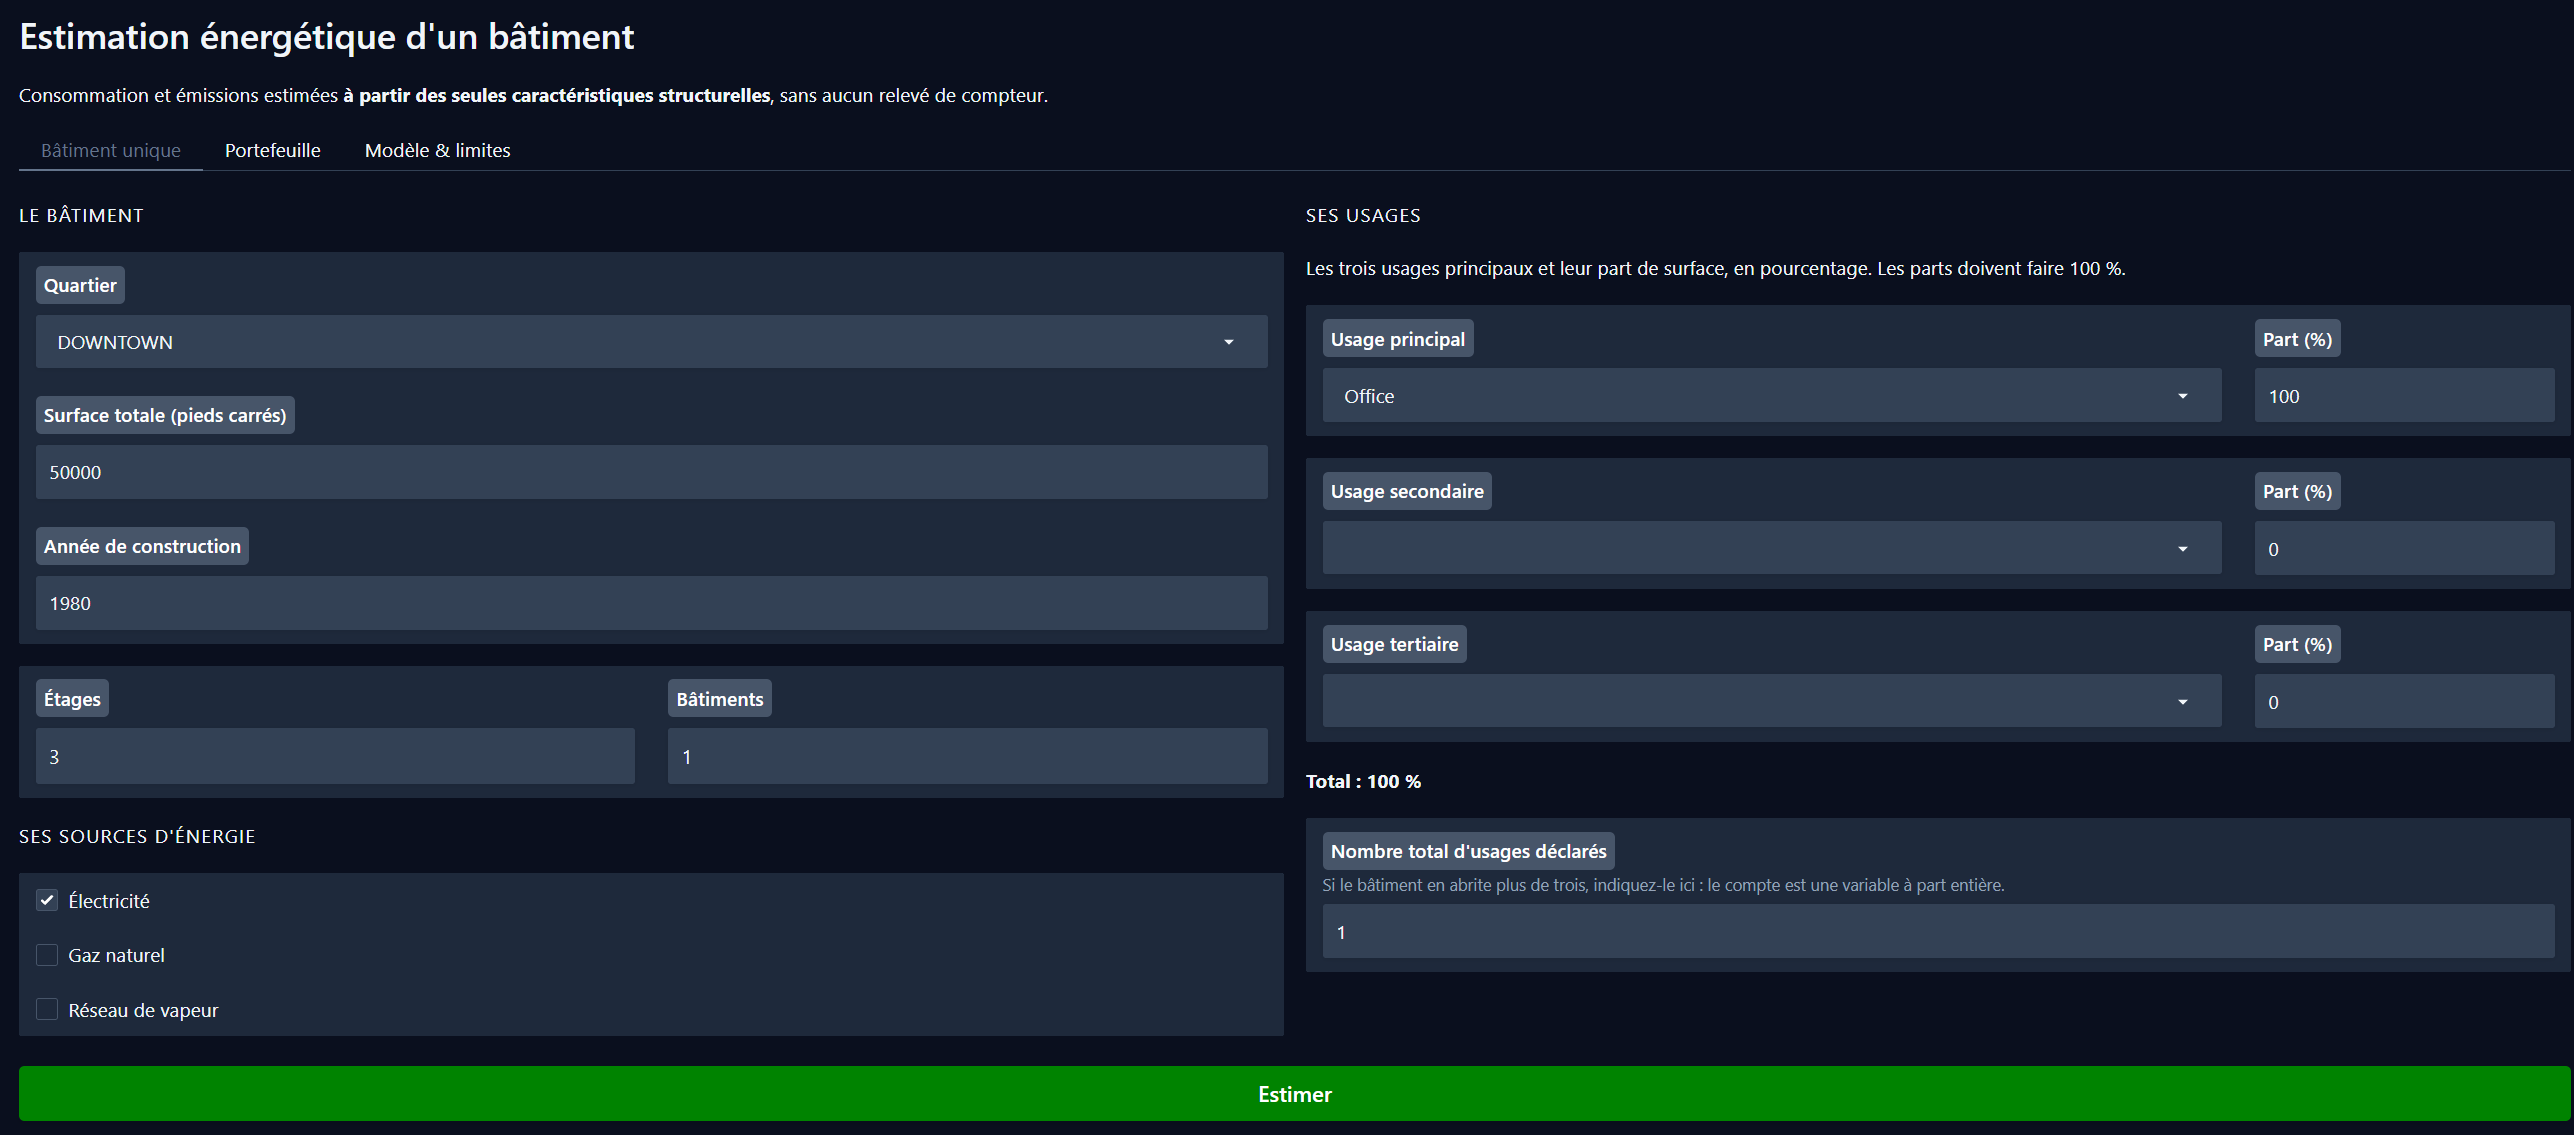
\includegraphics[width=\linewidth]{figures/app-batiment-saisie.png}
\caption{Saisie d'un bâtiment. Les parts d'usage sont contrôlées en direct :
l'interface collecte des pourcentages qui doivent totaliser 100~\%, et un champ
distinct porte le nombre total d'usages déclarés (écart E16).}
\end{figure}

\begin{figure}[ht]
\centering
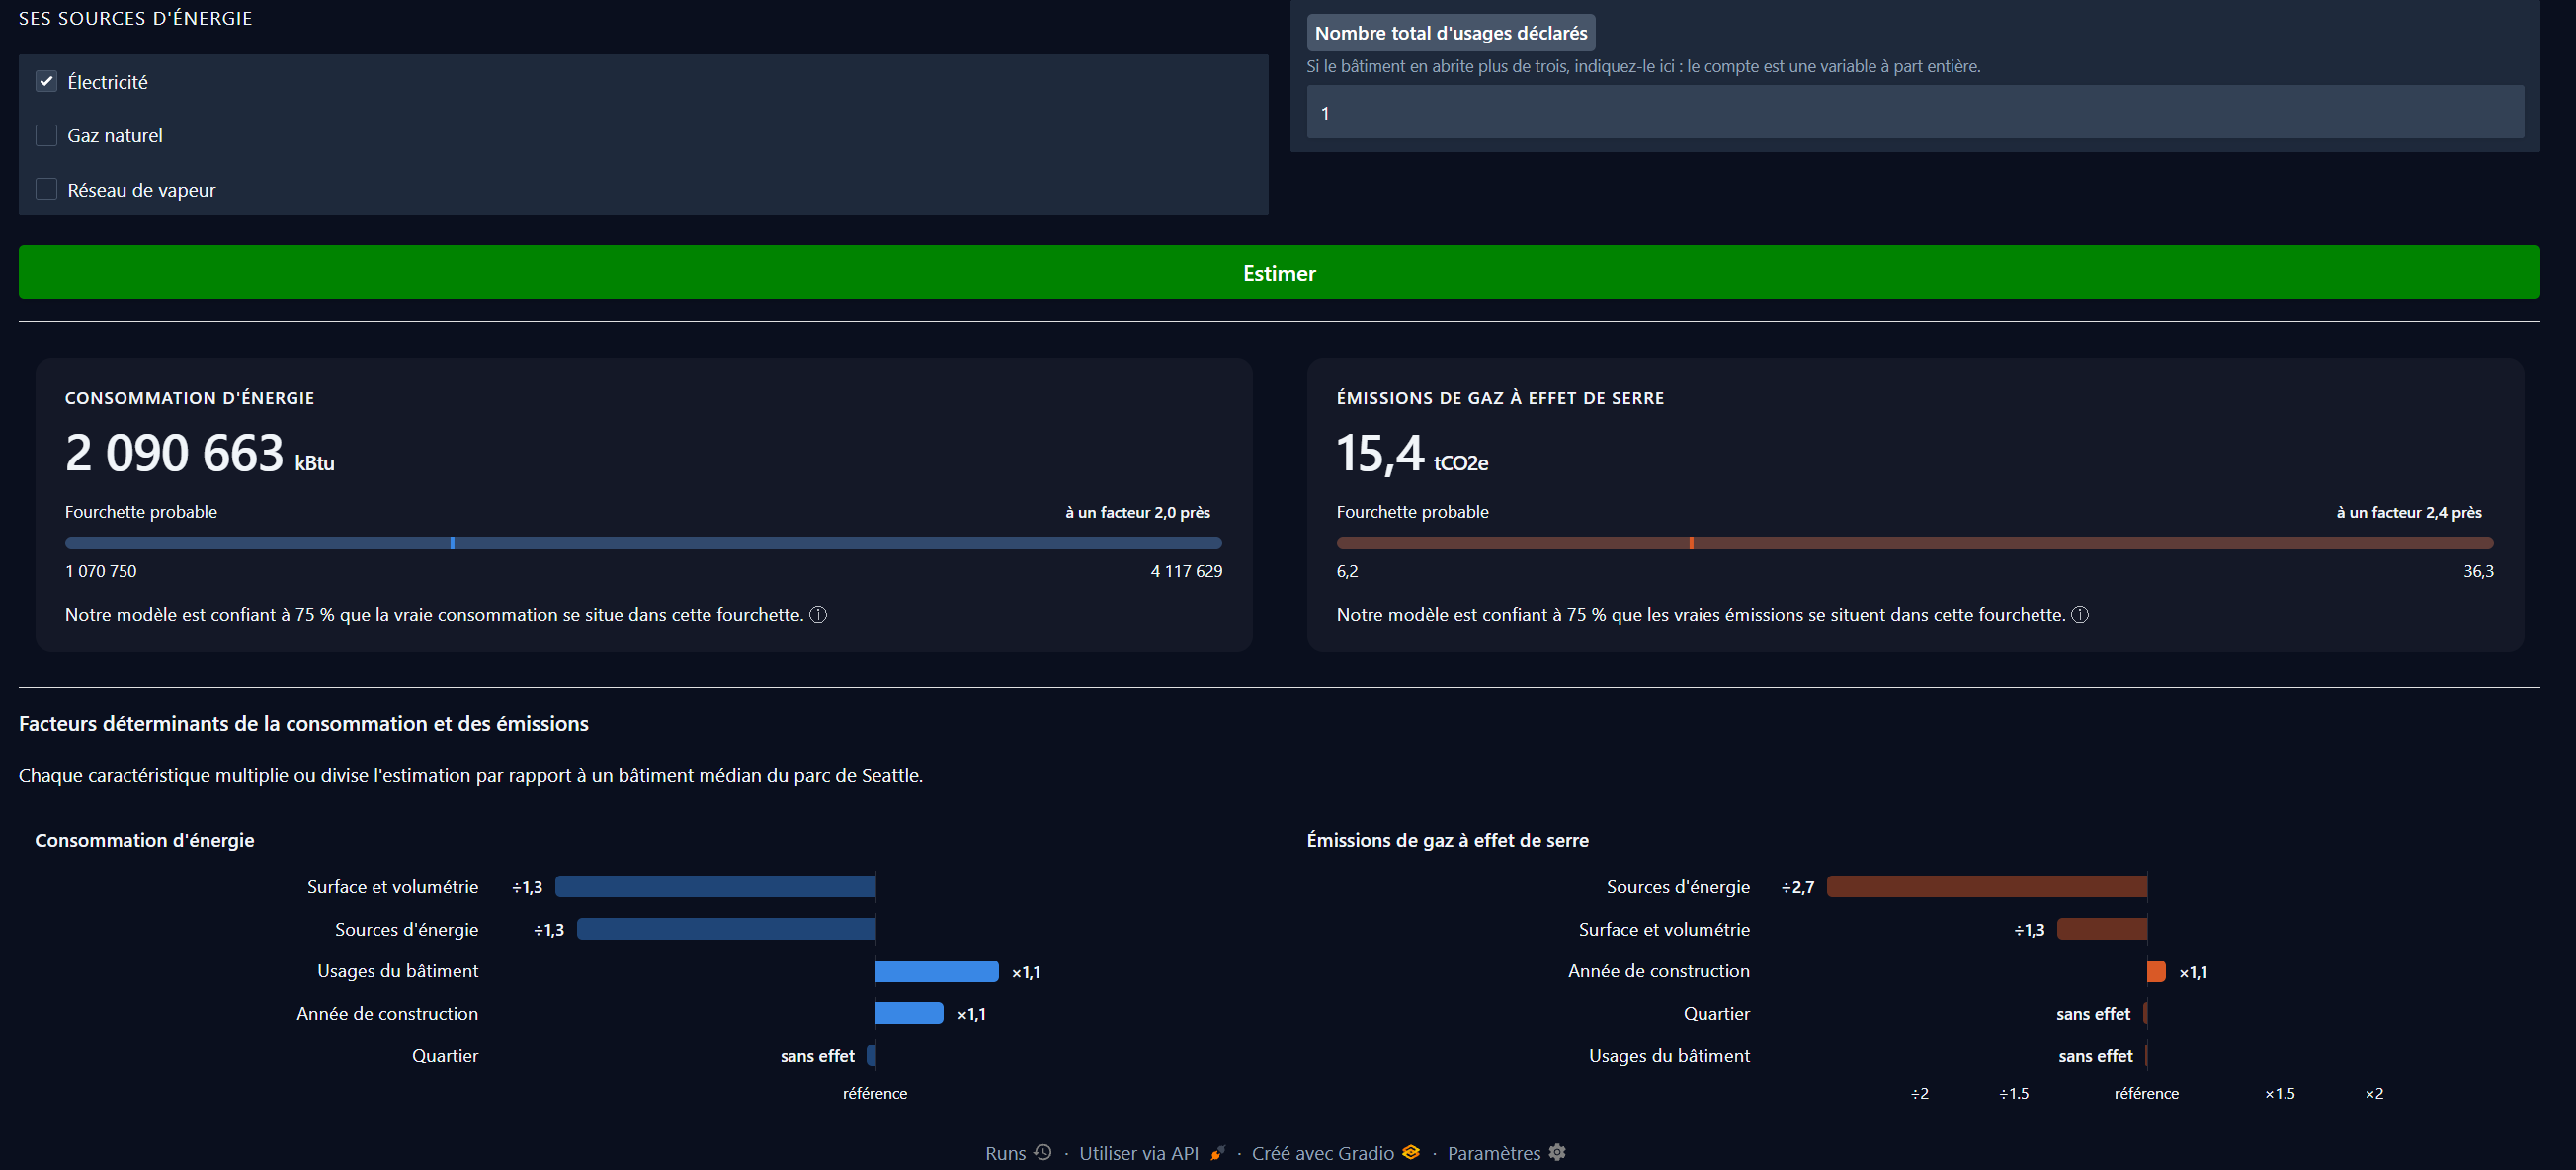
\includegraphics[width=\linewidth]{figures/app-batiment-resultats.png}
\caption{Résultat. La fourchette est donnée au même niveau que l'estimation, et
les contributions sont traduites en \emph{facteurs multiplicatifs} : le modèle
travaillant sur le logarithme de la cible, une contribution additive devient un
multiplicateur, forme directement lisible par un non-spécialiste.}
\end{figure}

\begin{figure}[ht]
\centering
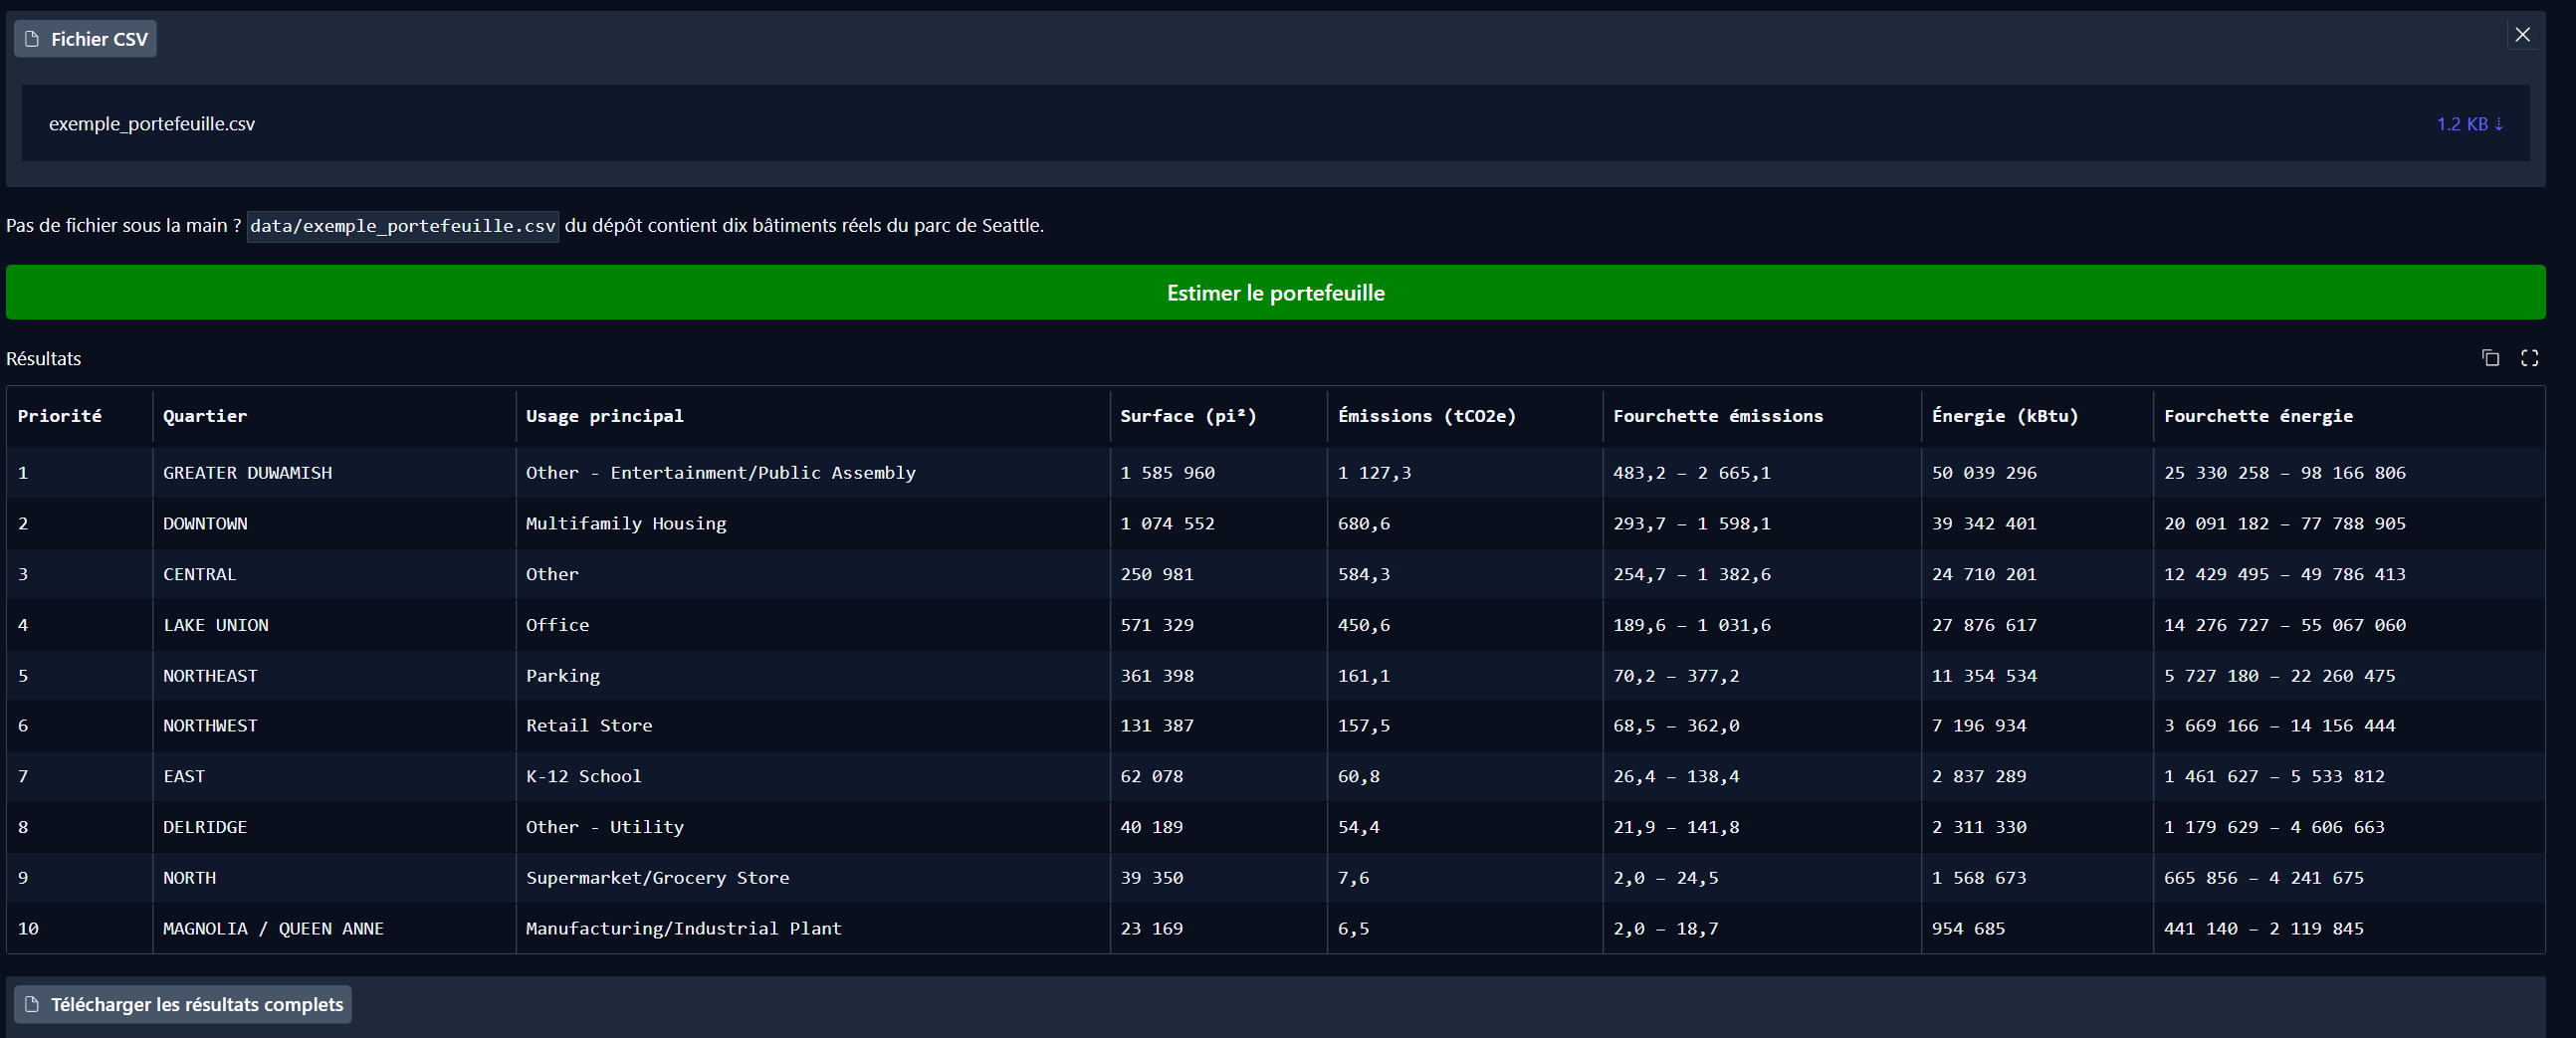
\includegraphics[width=\linewidth]{figures/app-portefeuille-tableau.png}
\caption{Portefeuille : le parc ressort trié par émissions estimées
décroissantes, c'est-à-dire dans l'ordre où lancer les audits.}
\end{figure}

\begin{figure}[ht]
\centering
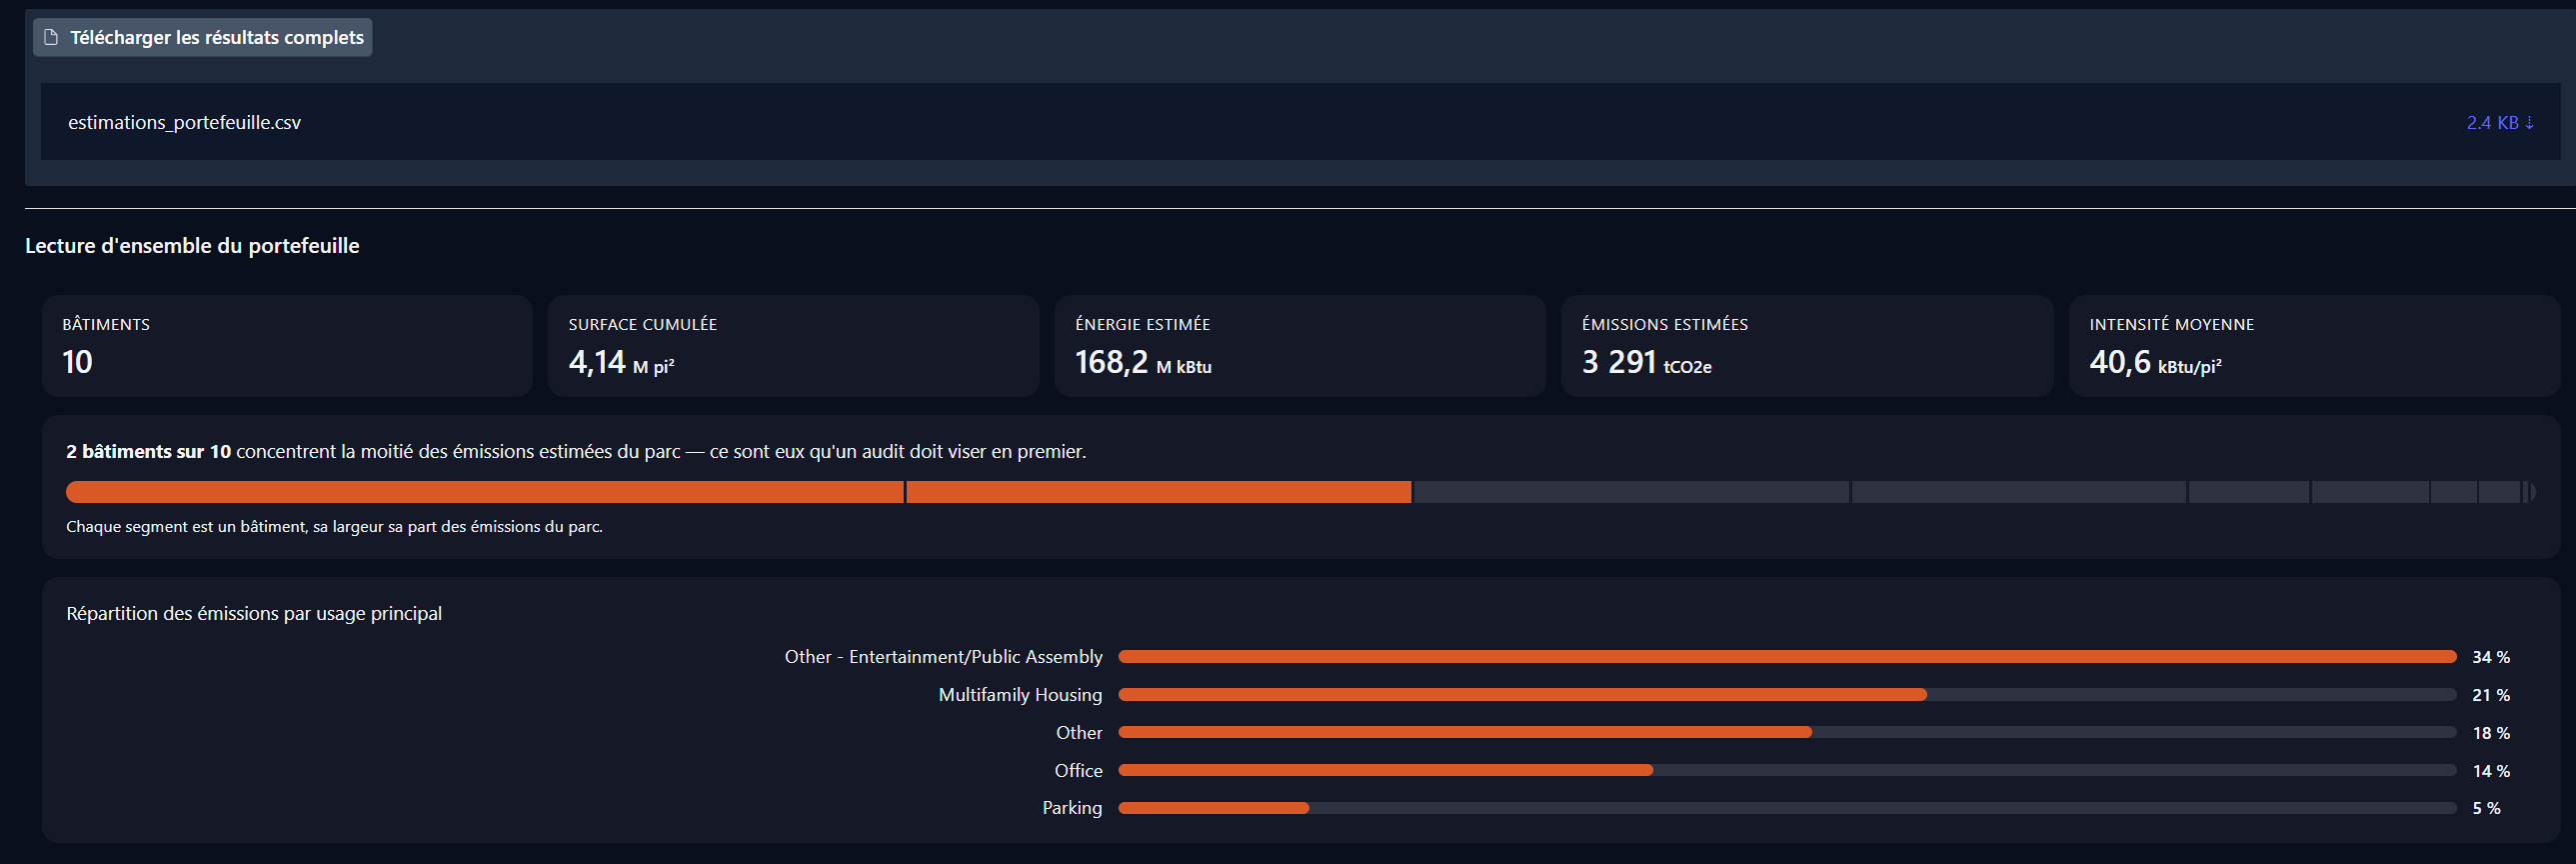
\includegraphics[width=\linewidth]{figures/app-portefeuille-synthese.png}
\caption{Synthèse de portefeuille. La barre de concentration est l'apport
principal de l'onglet : elle montre combien de bâtiments portent la moitié des
émissions du parc, ce qui transforme une liste en plan d'audit.}
\end{figure}

\subsection{Facteurs clés de succès et points de vigilance}

\begin{table}[H]
\centering
\small
\begin{tabularx}{\linewidth}{@{}L{4.6cm}X@{}}
\toprule
\textbf{Facteur clé de succès} & \textbf{Pourquoi} \\
\midrule
Préparation partagée & Élimine par construction l'écart entraînement / inférence \\
Fourchette systématique & Sans elle, l'estimation serait lue comme une mesure \\
Artefacts versionnés avec le code & 2,1~Mo : un téléchargement au démarrage n'ajouterait qu'un mode de panne \\
Versions épinglées sur celles de l'entraînement & Un modèle désérialisé par une autre version se dégrade sans erreur \\
\midrule
\textbf{Point de vigilance} & \textbf{Mesure de maîtrise} \\
\midrule
Dépendance à un hébergeur gratuit & Les conditions ont déjà changé deux fois ; le code reste portable \\
Domaine d'entraînement restreint & Un avertissement s'affiche hors du domaine, sans bloquer \\
Garantie de couverture marginale & Écrit dans l'onglet « modèle \& limites » plutôt que passé sous silence \\
Réentraînement annuel & Chaîne de tests exécutable avant tout redéploiement \\
\bottomrule
\end{tabularx}
\caption{Facteurs de succès et vigilances.}
\end{table}

\subsection{Méthodologie de priorisation des cas d'usage}

Trois cas d'usage ont été identifiés à partir des besoins de la
section~1.2, puis hiérarchisés selon la valeur métier et le coût de mise en
œuvre. Ils ont tous les trois été livrés, dans cet ordre.

\begin{table}[H]
\centering
\small
\begin{tabularx}{\linewidth}{@{}cL{3.6cm}XL{2.1cm}@{}}
\toprule
\textbf{Rang} & \textbf{Cas d'usage} & \textbf{Justification du rang} & \textbf{Livrable} \\
\midrule
1 & Priorisation d'un parc & Sert directement le besoin le plus valorisé ; un CSV suffit en entrée & Onglet portefeuille \\
2 & Estimation d'un bâtiment & Porte d'entrée pédagogique de l'outil et démonstrateur de la fourchette & Onglet bâtiment \\
3 & Explication d'une estimation & Nécessaire à l'acceptation, mais sans valeur seul & Facteurs multiplicatifs \\
\bottomrule
\end{tabularx}
\caption{Hiérarchisation des cas d'usage.}
\end{table}

\newpage

\section{Appui stratégique et méthodologique}
\markboth{4. Appui stratégique et méthodologique}{}

\subsection{Proposition de démarche projet}

\subsubsection*{Méthodologie retenue}

La démarche suit \textbf{CRISP-DM}, avec une adaptation : la phase de déploiement
n'est pas un aboutissement mais une contrainte amont. Le besoin « servir un
bâtiment non relevé » a été posé \emph{avant} la modélisation, et c'est lui qui a
disqualifié les variables en fuite. Une démarche où le déploiement arrive en
dernier aurait laissé la fuite passer jusqu'en production.

Le cycle est itératif dans les faits : la découverte de la fuite en phase de
préparation a provoqué un retour en compréhension du métier, et la contrainte
d'hébergement rencontrée en phase de déploiement a provoqué un retour en
conception.

\subsubsection*{Feuille de route}

\begin{table}[H]
\centering
\small
\begin{tabularx}{\linewidth}{@{}L{1.3cm}L{3.4cm}XL{2.4cm}@{}}
\toprule
\textbf{Phase} & \textbf{Objet} & \textbf{Livrable de sortie} & \textbf{Jalon} \\
\midrule
0 & Cadrage & Plan de travail, dépôt initialisé, règle de traçabilité & Périmètre arrêté \\
1 & Reprise et audit des données & Jeu nettoyé, journal d'écarts ouvert & Données rejouables \\
2 & Préparation partagée & \code{src/features.py}, analyse bivariée & Préparation figée \\
3 & Modélisation et arbitrages & Banc d'essai, conformalisation, artefacts & Modèles exportés \\
4 & Application & Interface, trois cas d'usage & Application locale \\
5 & Industrialisation & Tests, CI/CD, déploiement & \textbf{Application en ligne} \\
6 & Restitution & Rapport, portfolio & Soutenance \\
\bottomrule
\end{tabularx}
\caption{Feuille de route par phases.}
\end{table}

\subsubsection*{Responsabilités}

Le projet est conduit par une personne seule, ce qui n'annule pas la question des
rôles mais la déplace : chaque rôle doit être \emph{explicitement endossé} à un
moment donné, faute de quoi il est oublié.

\begin{table}[H]
\centering
\small
\begin{tabularx}{\linewidth}{@{}L{3.4cm}X@{}}
\toprule
\textbf{Rôle endossé} & \textbf{Ce qu'il a effectivement produit} \\
\midrule
Analyste métier & Reconstitution des besoins, matrice de priorisation, périmètre \\
Auditeur & Grille d'évaluation de l'existant, mise en évidence de la fuite \\
Data scientist & Préparation, banc d'essai, conformalisation \\
Ingénieur MLOps & Tests, CI/CD, versionnement des artefacts, déploiement \\
Concepteur d'interface & Hiérarchie visuelle, formulation métier de l'incertitude \\
\bottomrule
\end{tabularx}
\caption{Rôles endossés au cours du projet.}
\end{table}

\subsection{Aide à la prise de décision}

\subsubsection*{Risques et opportunités}

\begin{table}[H]
\centering
\small
\begin{tabularx}{\linewidth}{@{}L{4.4cm}L{1.6cm}X@{}}
\toprule
\textbf{Risque} & \textbf{Gravité} & \textbf{Réponse apportée} \\
\midrule
Estimation prise pour une mesure & \textbf{Élevée} & Fourchette systématique, usage écrit dans l'interface \\
Dérive de versions entre entraînement et service & \textbf{Élevée} & Versions épinglées et vérifiées par un test dédié \\
Changement des conditions de l'hébergeur & Moyenne & Déjà survenu deux fois ; le code reste portable \\
Bâtiment hors domaine soumis à l'outil & Moyenne & Avertissement non bloquant au-delà du domaine observé \\
Réentraînement dégradant le modèle & Moyenne & Seuils de non-régression bloquants en intégration continue \\
Abandon de maintenance & Faible & Aucune brique à surveiller en continu, par conception \\
\midrule
\textbf{Opportunité} & & \textbf{Condition de réalisation} \\
\midrule
API réutilisable par un tiers & & Acquise, générée par le cadre applicatif \\
Extension à d'autres millésimes & & Le pipeline est rejouable ; coût marginal faible \\
Extension à d'autres villes & & \textbf{Non} : romprait l'hypothèse d'échangeabilité \\
\bottomrule
\end{tabularx}
\caption{Synthèse des risques et opportunités.}
\end{table}

\subsubsection*{Scénarios budgétaires}

Les coûts d'infrastructure sont documentés ci-dessous. Le coût de mise en œuvre
est exprimé en jours-homme ; sa valorisation dépend du taux journalier retenu et
n'est donc pas chiffrée ici.

\begin{table}[H]
\centering
\small
\begin{tabularx}{\linewidth}{@{}L{3.2cm}L{2.4cm}XL{2.2cm}@{}}
\toprule
\textbf{Scénario} & \textbf{Coût récurrent} & \textbf{Ce qu'il apporte} & \textbf{Décision} \\
\midrule
Hébergement gratuit & \textbf{0\,\$} & Application publique, mise en veille automatique après inactivité & \textbf{Retenu} \\
\addlinespace
Abonnement PRO & 9\,\$ / mois & Débloque le conteneur Docker et le matériel CPU dédié & Écarté : n'achète qu'une différence d'outillage \\
\addlinespace
Matériel CPU dédié & $\approx$ 22\,\$ / mois & Supprime le temps de démarrage à froid & Écarté : voir ci-dessous \\
\bottomrule
\end{tabularx}
\caption{Scénarios budgétaires d'infrastructure.}
\end{table}

\begin{constat}{Un arbitrage éclairé par la mesure d'empreinte}
Le troisième scénario a été écarté sur un argument qui n'est pas seulement
financier. Un conteneur maintenu éveillé consomme, à 10~W de puissance moyenne,
environ \textbf{88~kWh par an} — soit \textbf{douze mille fois} l'énergie
consommée par la totalité du banc d'essai. Pour un modèle réentraîné une fois par
an et un usage épisodique, payer pour supprimer un temps de démarrage revient à
financer une consommation continue sans contrepartie d'usage.
\end{constat}

\subsubsection*{Indicateurs de succès}

\begin{table}[H]
\centering
\small
\begin{tabularx}{\linewidth}{@{}L{4.8cm}L{3.2cm}X@{}}
\toprule
\textbf{Indicateur} & \textbf{Cible} & \textbf{Nature} \\
\midrule
Erreur relative médiane hors bloc & $\leq 40\,\%$ & Technique, bloquant en CI \\
Couverture observée des fourchettes & $\geq 75\,\%$ & Technique, bloquant en CI \\
Bornes ordonnées sur tout le parc & 100\,\% & Technique, bloquant en CI \\
Suite de tests au vert avant déploiement & 100\,\% & Technique, bloquant \\
\midrule
Part des émissions couverte par les 20\,\% premiers audits & À mesurer & Métier \\
Taux de confirmation d'une priorisation par l'audit réel & À mesurer & Métier \\
Nombre de bâtiments pré-qualifiés sans déplacement & À mesurer & Métier \\
\bottomrule
\end{tabularx}
\caption{Indicateurs de succès techniques et métier.}
\end{table}

Les indicateurs métier sont marqués « à mesurer » et non renseignés : ils
supposent un retour d'usage qui n'existe pas encore. Les afficher avec des
valeurs inventées les rendrait inutiles.

\subsubsection*{Impacts pris en compte}

\begin{description}[leftmargin=0em,style=nextline,itemsep=0.35em]
  \item[Éthique et réputationnel] Les données sont publiques et nominatives à
        l'échelle du bâtiment. Publier qu'un bâtiment identifié est « le plus
        consommateur de sa catégorie » sur la foi d'une estimation fausse d'un
        facteur~2 serait dommageable pour son propriétaire. C'est la raison
        première pour laquelle la fourchette est affichée au même niveau que
        l'estimation, et non en note de bas de page.
  \item[Légal] Les estimations sont opposables dans un contexte réglementaire.
        L'interface indique explicitement qu'elles ne peuvent servir ni à
        facturer, ni à contractualiser, ni à dimensionner un investissement.
  \item[Données personnelles] Aucune donnée à caractère personnel n'est traitée :
        le jeu décrit des bâtiments, pas des occupants. Le RGPD n'est pas
        applicable au traitement.
  \item[Environnemental] L'empreinte de l'entraînement a été mesurée plutôt
        qu'estimée, et cette mesure a servi un arbitrage réel
        (section~\ref{sec:carbone}).
  \item[Organisationnel] La solution n'ajoute aucune brique à surveiller en
        continu, ce qui est une décision de conception assumée pour un service
        disposant d'un seul utilisateur métier et d'aucune équipe d'exploitation.
\end{description}

\newpage

\section{Contrôle et suivi du projet}
\markboth{5. Contrôle et suivi du projet}{}

\subsection{Tableau de bord de pilotage}

\subsubsection*{Indicateurs suivis}

\begin{table}[H]
\centering
\small
\begin{tabularx}{\linewidth}{@{}L{2.5cm}L{4.6cm}XL{2.1cm}@{}}
\toprule
\textbf{Dimension} & \textbf{Indicateur} & \textbf{Valeur au terme du projet} & \textbf{Fréquence} \\
\midrule
Délais & Phases achevées & 6 sur 6 & Par phase \\
Coûts & Coût d'infrastructure récurrent & 0\,\$ & Mensuelle \\
Livrables & Application, dépôt, tests, rapport & Livrés & Par phase \\
\midrule
Qualité des données & Lignes retenues après nettoyage & \num{1655} sur \num{1656} & Par millésime \\
& Écarts documentés vis-à-vis de l'existant & 16 & Au fil de l'eau \\
& Modalités inconnues acceptées silencieusement & 0 (exception levée) & Continu \\
\midrule
Performance ML & $R^2$ hors bloc, énergie & 0,745 & Par réentraînement \\
& $R^2$ hors bloc, émissions & 0,723 & Par réentraînement \\
& Erreur relative médiane & 36,6\,\% / 45,1\,\% & Par réentraînement \\
& Couverture observée des fourchettes & 81,3\,\% / 81,0\,\% & Par réentraînement \\
\midrule
Qualité logicielle & Tests automatisés & 61, tous au vert & À chaque \emph{commit} \\
& Analyse statique & Sans avertissement & À chaque \emph{commit} \\
\midrule
Empreinte & Énergie du banc d'essai complet & 7,3~Wh & Par campagne \\
\bottomrule
\end{tabularx}
\caption{Tableau de bord de pilotage.}
\end{table}

\subsubsection*{Mode de reporting}

Trois canaux, chacun avec sa fréquence propre :

\begin{description}[leftmargin=0em,style=nextline,itemsep=0.3em]
  \item[À chaque \emph{commit}] La chaîne d'intégration continue exécute l'analyse
        statique puis les tests. Un échec bloque le déploiement — le reporting
        est ici un verrou, pas une information.
  \item[À chaque campagne de modélisation] Le registre d'expérimentations
        enregistre paramètres, métriques et empreinte. Aucune comparaison de
        modèles ne repose sur un chiffre recopié à la main.
  \item[Au fil de l'eau] Le journal d'écarts reçoit une ligne \emph{au moment} du
        changement, jamais après coup. C'est ce qui rend la section~2 de ce
        rapport rédigeable sans reconstitution a posteriori.
\end{description}

\subsection{Outils et process de suivi}

\subsubsection*{Suivi des expérimentations}

\textbf{26 exécutions} ont été enregistrées : douze modèles évalués sous deux
protocoles — avec et sans les variables en fuite — plus les deux modèles de
production. Chaque exécution porte ses paramètres, ses métriques, sa durée et son
empreinte carbone.

Les deux modèles retenus sont inscrits au registre de modèles avec un alias
\code{@champion}, ce qui rend la sélection auditable : on peut répondre à la
question « pourquoi ce modèle-ci ? » par une trace, pas par un souvenir.

\begin{constat}{Ce que le suivi a réellement servi}
Sans registre, la comparaison « avec ratios / sans ratios » aurait été une
impression. Avec, elle est un tableau : la fuite coûte $9{,}7$~points sur les
émissions et $1{,}3$~point sur l'énergie. C'est ce chiffre qui a permis
d'\emph{assumer} la baisse de performance auprès d'un lecteur qui n'y aurait vu
qu'une régression.
\end{constat}


\begin{figure}[ht]
\centering
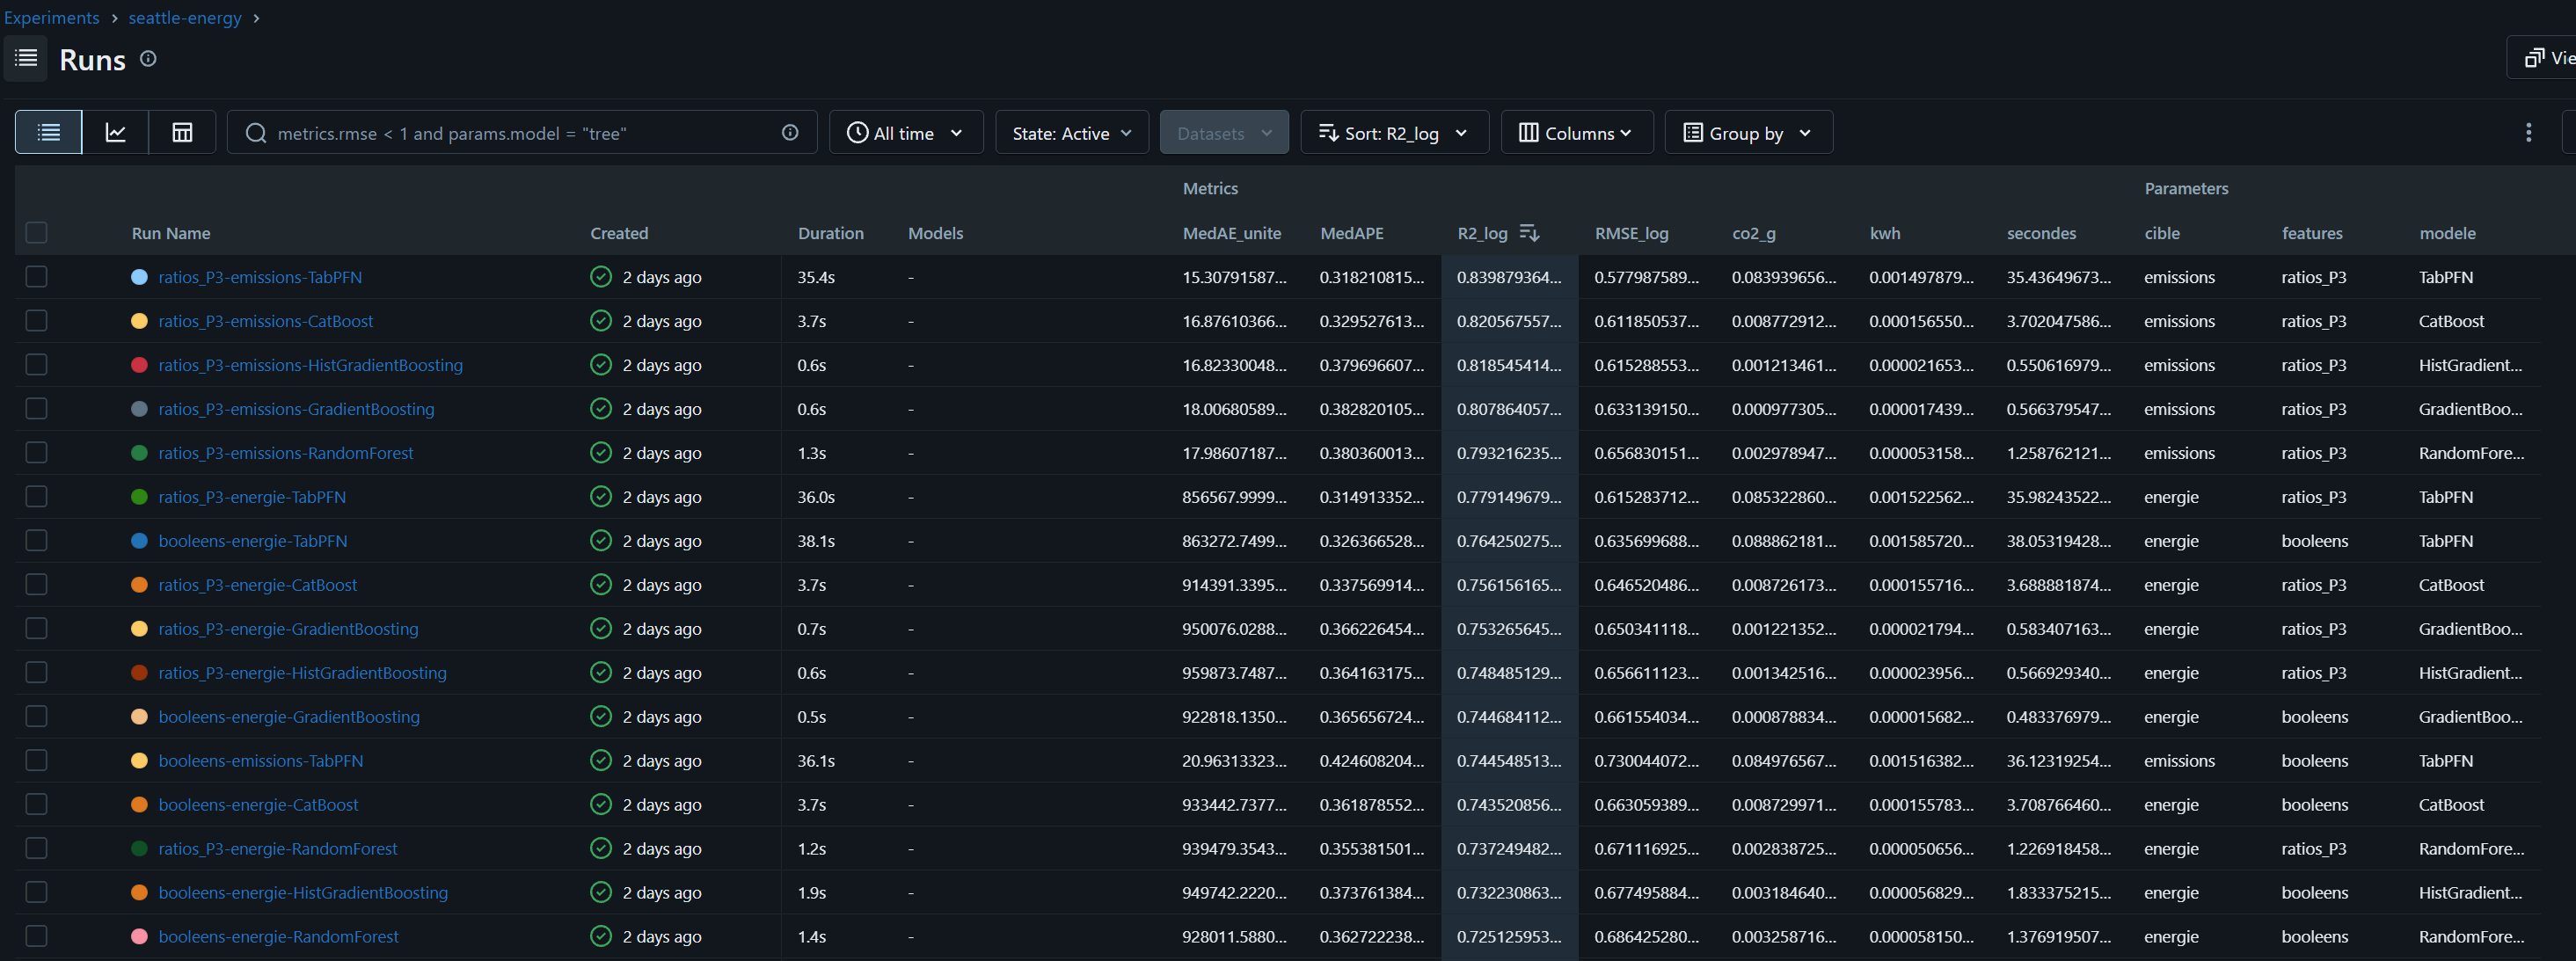
\includegraphics[width=\linewidth]{figures/mlflow-runs.png}
\caption{Registre d'expérimentations. Chaque exécution porte ses métriques, sa
durée et son empreinte, ce qui rend la comparaison « avec ratios / sans ratios »
vérifiable plutôt qu'affirmée.}
\end{figure}

\subsubsection*{Intégration et déploiement continus}

\begin{table}[H]
\centering
\small
\begin{tabularx}{\linewidth}{@{}L{3.6cm}X@{}}
\toprule
\textbf{Étape} & \textbf{Rôle} \\
\midrule
Analyse statique & Style et erreurs détectables sans exécution \\
Suite de tests & 61 tests : préparation, invariants du modèle, interface, configuration de déploiement \\
Déploiement conditionnel & Uniquement sur la branche principale, uniquement si tout est vert \\
\bottomrule
\end{tabularx}
\caption{Chaîne d'intégration et de déploiement.}
\end{table}

Un choix mérite d'être signalé : la chaîne installe les dépendances \textbf{depuis le
fichier de dépendances de l'application}, et non depuis l'environnement de
développement. La suite valide donc les artefacts contre la pile exacte que le
service fera tourner, et non contre celle du poste du développeur.


\begin{figure}[ht]
\centering
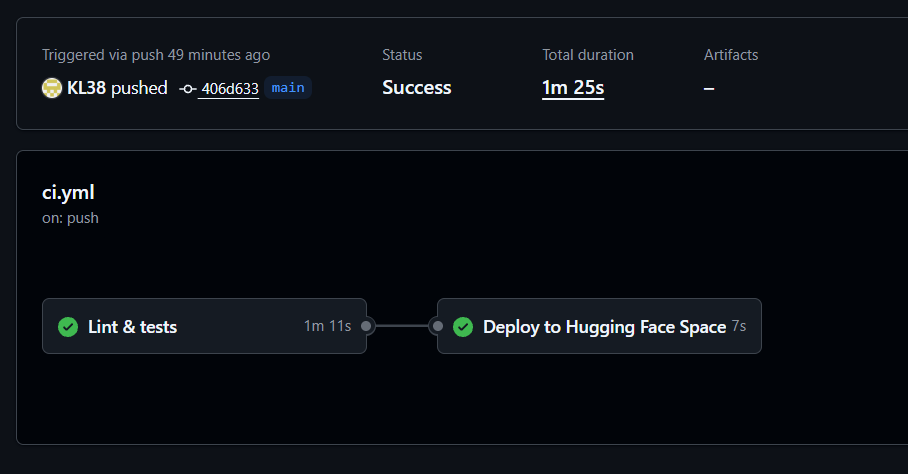
\includegraphics[width=0.78\linewidth]{figures/cicd-jobs.png}
\caption{Un cycle complet : les tests conditionnent le déploiement, qui ne
s'exécute que sur la branche principale.}
\end{figure}

\begin{figure}[ht]
\centering
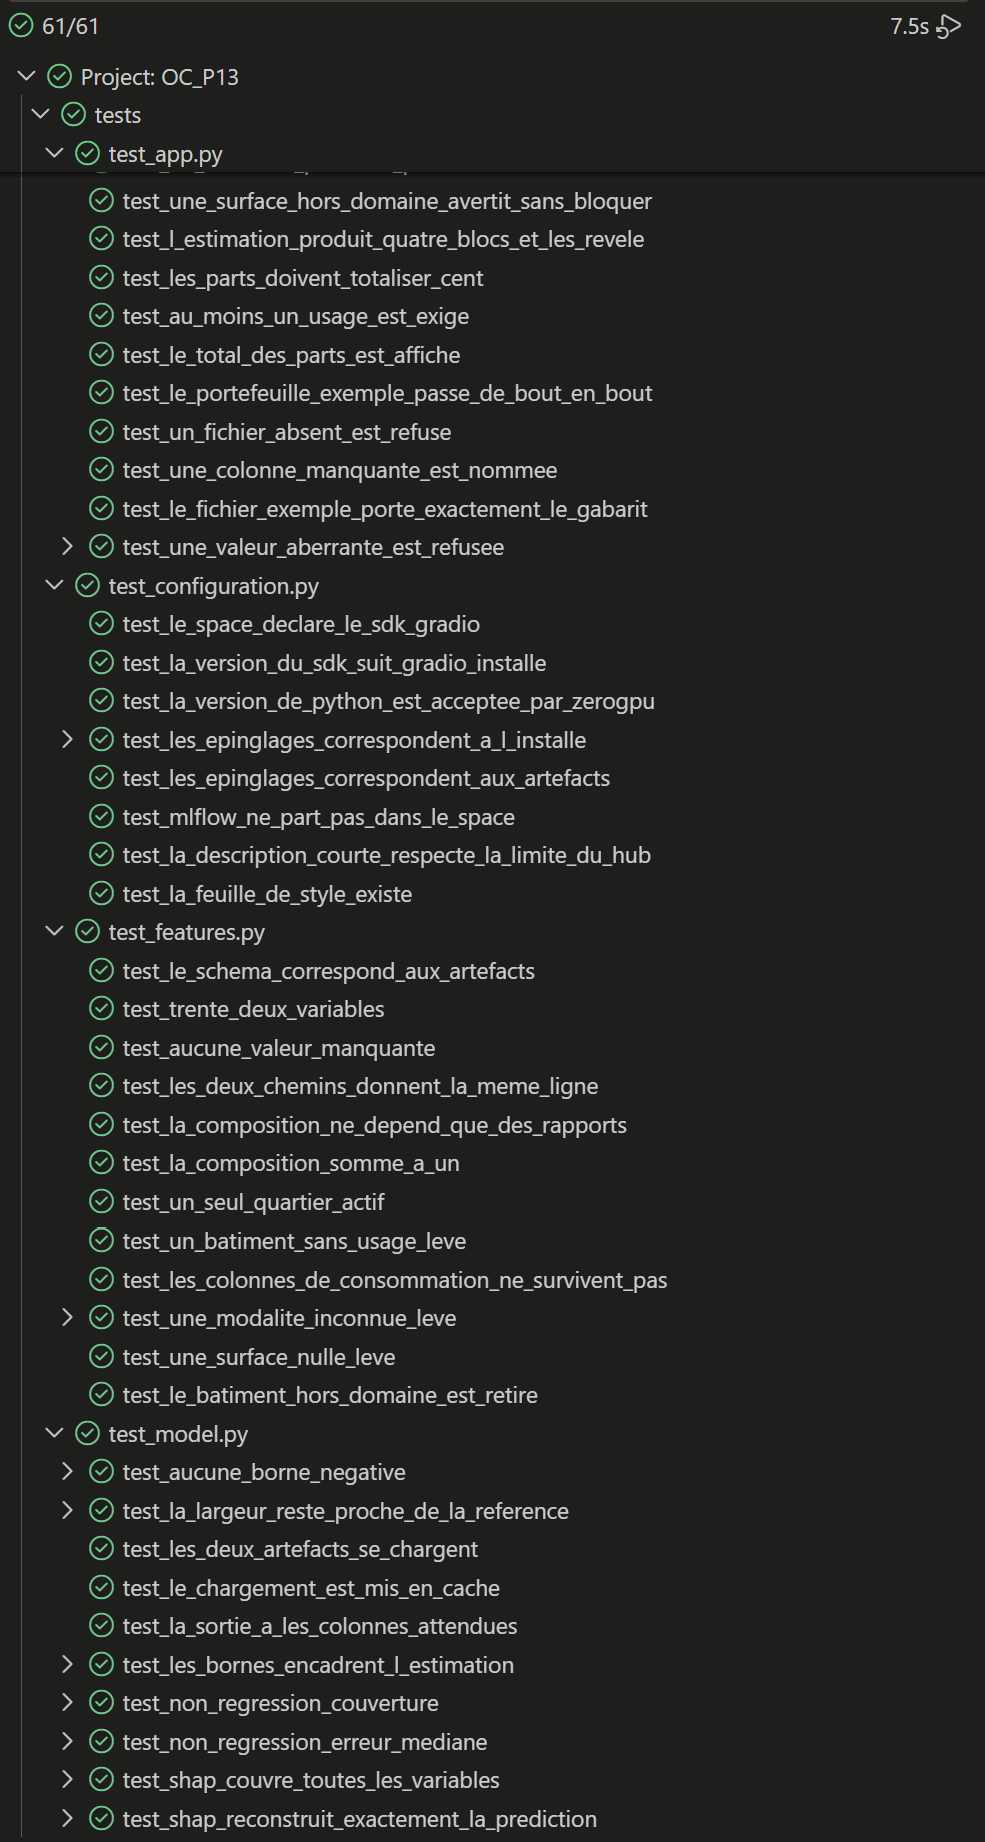
\includegraphics[height=13.5cm]{figures/tests-suite.png}
\caption{La suite de tests. Les quatre fichiers couvrent la préparation des
données, les invariants du modèle, les points d'entrée de l'interface et la
configuration de déploiement.}
\end{figure}

\subsubsection*{Trois défauts réels attrapés par le dispositif}

Le dispositif de contrôle n'est pas décoratif : il a produit trois constats que
la relecture humaine n'avait pas produits.

\begin{enumerate}[leftmargin=1.6em,itemsep=0.45em]
  \item \textbf{Une borne négative en production.} Un bâtiment sur \num{1655}
        sortait avec une borne basse d'émissions à $-0{,}134$~tCO\textsubscript{2}e.
        La cause est structurelle : la cible étant transformée en logarithme, la
        soustraction du quantile de conformité passe sous zéro pour une valeur
        minuscule. Corrigé par une projection sur le domaine physiquement
        admissible, sans perte de couverture.
  \item \textbf{Une dérive d'environnement.} L'exécution des tests depuis un
        environnement Python différent a révélé une bibliothèque d'apprentissage
        en version~1.8 alors que les artefacts avaient été produits en~1.9.
        Servi ainsi, le modèle aurait été désérialisé par une version autre que
        celle qui l'a ajusté — sans erreur ni avertissement. C'est le mode de
        panne silencieux que le test de configuration a été écrit pour attraper.
  \item \textbf{Une contrainte de plateforme non documentée.} Le déploiement a
        échoué sur une limite de longueur d'un champ de métadonnées, refusée non
        pas au niveau du champ mais de \emph{tout l'envoi}, après que les tests
        soient passés au vert. Un test vérifie désormais cette contrainte en
        amont.
\end{enumerate}

\subsubsection{Empreinte carbone : une mesure qui a tranché}
\label{sec:carbone}

L'empreinte de chaque entraînement a été mesurée modèle par modèle. Le résultat
utile n'est pas le total, il est dans les rapports.

\begin{table}[H]
\centering
\small
\begin{tabular}{@{}lrrr@{}}
\toprule
\textbf{Modèle} & \textbf{Durée} & \textbf{Énergie} & \textbf{$R^2$ énergie} \\
\midrule
GradientBoosting & 0,48~s & \textbf{0,016~Wh} & 0,745 \\
RandomForest & 1,38~s & 0,058~Wh & 0,725 \\
CatBoost & 3,71~s & 0,156~Wh & 0,744 \\
TabPFN & 38,05~s & \textbf{1,586~Wh} & 0,764 \\
\bottomrule
\end{tabular}
\caption{Consommation par modèle, cible énergie.}
\end{table}

\begin{constat}{Le seul arbitrage que la mesure a réellement tranché}
TabPFN consomme à lui seul \textbf{84\,\%} de l'énergie du banc d'essai complet,
soit \textbf{101 fois} le modèle retenu, pour un gain de deux points dans le bruit
d'échantillonnage. Il était déjà écarté pour sa licence ; la mesure lui donne un
\textbf{second motif de rejet, indépendant du premier}.
\end{constat}


\begin{figure}[ht]
\centering
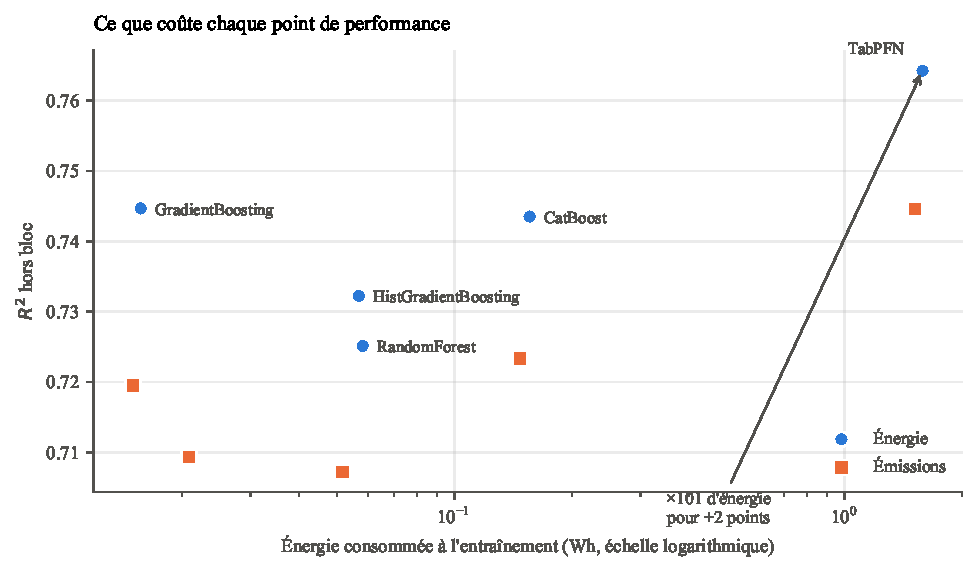
\includegraphics[width=\linewidth]{figures/empreinte-performance.pdf}
\caption{Coût énergétique de chaque point de performance. L'échelle des abscisses
est logarithmique : les cinq premiers modèles tiennent dans une décade, TabPFN
seul en occupe deux de plus.}
\end{figure}

Trois limites de l'indicateur sont documentées plutôt que passées sous silence :

\begin{itemize}[leftmargin=1.4em,itemsep=0.2em]
  \item \textbf{En absolu, la mesure n'arbitre rien.} Le banc d'essai complet a
        consommé 7,3~Wh et émis 0,41~g de CO\textsubscript{2}e — l'équivalent
        d'une ampoule LED allumée trois quarts d'heure.
  \item \textbf{Sous deux secondes, elle n'est pas reproductible.} Entre deux
        campagnes, les modèles les plus rapides varient de $+39\,\%$ et
        $-58\,\%$, quand les plus longs tiennent à quelques pourcents près.
  \item \textbf{Le lieu pèse plus que le modèle.} Le facteur de conversion mesuré
        est de 56~g\,CO\textsubscript{2}/kWh (mix français) ; sur un mix
        nord-américain le même calcul émettrait cinq à sept fois plus. Un chiffre
        d'empreinte n'est comparable qu'à un autre produit sur la même
        infrastructure.
\end{itemize}

\subsubsection{Le dispositif volontairement non implémenté}
\label{sec:monitoring}

Aucune supervision de dérive n'a été mise en place, et c'est une décision, pas un
oubli. Les données sont publiées une fois par an, le modèle est réentraîné au
même rythme, et le service compte un seul utilisateur métier sans équipe
d'exploitation. Une brique de supervision aurait ajouté un service à héberger, à
authentifier et à maintenir, pour détecter une dérive dont la fréquence
d'apparition est celle du réentraînement lui-même.

\begin{constat}{Ce que coûte une bonne pratique appliquée sans discernement}
Le coût de maintenance aurait dépassé le bénéfice attendu. L'arbitrage est
documenté ici précisément parce qu'un lecteur pourrait y voir une lacune : c'est
l'absence de justification, et non l'absence de l'outil, qui constituerait le
défaut.
\end{constat}

\newpage

\section{Conclusion et recommandations}
\markboth{6. Conclusion et recommandations}{}

\subsection{Récapitulatif des décisions}

\begin{table}[H]
\centering
\small
\begin{tabularx}{\linewidth}{@{}L{4.2cm}XL{2.6cm}@{}}
\toprule
\textbf{Décision} & \textbf{Fondement} & \textbf{Nature} \\
\midrule
Supprimer les variables en fuite & Un utilisateur capable de les renseigner n'a pas besoin du modèle & Structurante \\
Accompagner toute estimation d'une fourchette & Un nombre seul est lu comme une mesure & Structurante \\
Fixer le niveau de confiance à 75\,\% & Au-delà, la fourchette cesse d'être exploitable & Arbitrage produit \\
Écarter TabPFN & Licence \emph{et} 101 fois l'énergie pour un gain dans le bruit & Sur mesure \\
Écarter la régression quantile conformalisée & Gain de couverture conditionnelle dans le bruit & Sur mesure \\
Écarter \code{ParkingRatio} & Confirme un arbitrage de la solution auditée & Sur mesure \\
Basculer vers Gradio & Seul chemin gratuit après changement des conditions de l'hébergeur & Contrainte subie \\
Ne pas écrire de \code{Dockerfile} & Non déployé, il aurait constitué une dette & Arbitrage assumé \\
Ne pas superviser la dérive & Coût de maintenance $>$ bénéfice à cette échelle & Arbitrage assumé \\
Versionner les artefacts avec le code & 2,1~Mo : un téléchargement n'ajouterait qu'un mode de panne & Technique \\
\bottomrule
\end{tabularx}
\caption{Décisions prises et leur fondement.}
\end{table}

\subsection{Le plafond de performance}

Le résultat le plus solide du projet est une limite, et il détermine à lui seul
où se trouvent les marges de progression.

\subsubsection*{La mesure}

On regroupe les bâtiments que le modèle voit comme \emph{interchangeables} —
même groupe d'usage dominant, même tranche de surface — et on observe la
dispersion réelle de leur intensité énergétique. Cet écart est irréductible :
aucun modèle utilisant ces variables ne peut le prédire.

\begin{table}[H]
\centering
\small
\begin{tabular}{@{}lrrrr@{}}
\toprule
\textbf{Groupe comparable} & \textbf{$n$} & \textbf{$p_{10}$} & \textbf{$p_{90}$} & \textbf{Rapport} \\
\midrule
Bureaux, grande tranche & 163 & 27,2 & 90,9 & \textbf{3,35} \\
Bureaux, tranche moyenne & 120 & 31,4 & 105,3 & 3,35 \\
Entrepôts secs & 69 & 9,8 & 71,0 & \textbf{7,27} \\
Salles et assemblées & 70 & 14,6 & 99,7 & 6,83 \\
Enseignement & 62 & 24,9 & 61,5 & 2,47 \\
\bottomrule
\end{tabular}
\caption{Dispersion de l'intensité (kBtu/pi²) entre bâtiments indiscernables.}
\end{table}

\begin{constat}{Le modèle est au plafond}
Une fourchette construite sur cette seule dispersion irréductible, au même niveau
de confiance, vaudrait un facteur \textbf{2,24}. Le modèle produit un facteur
\textbf{2,03}. Il est donc \emph{plus serré} que l'écart naturel entre bâtiments
que les données ne permettent pas de distinguer.
\end{constat}


\begin{figure}[ht]
\centering
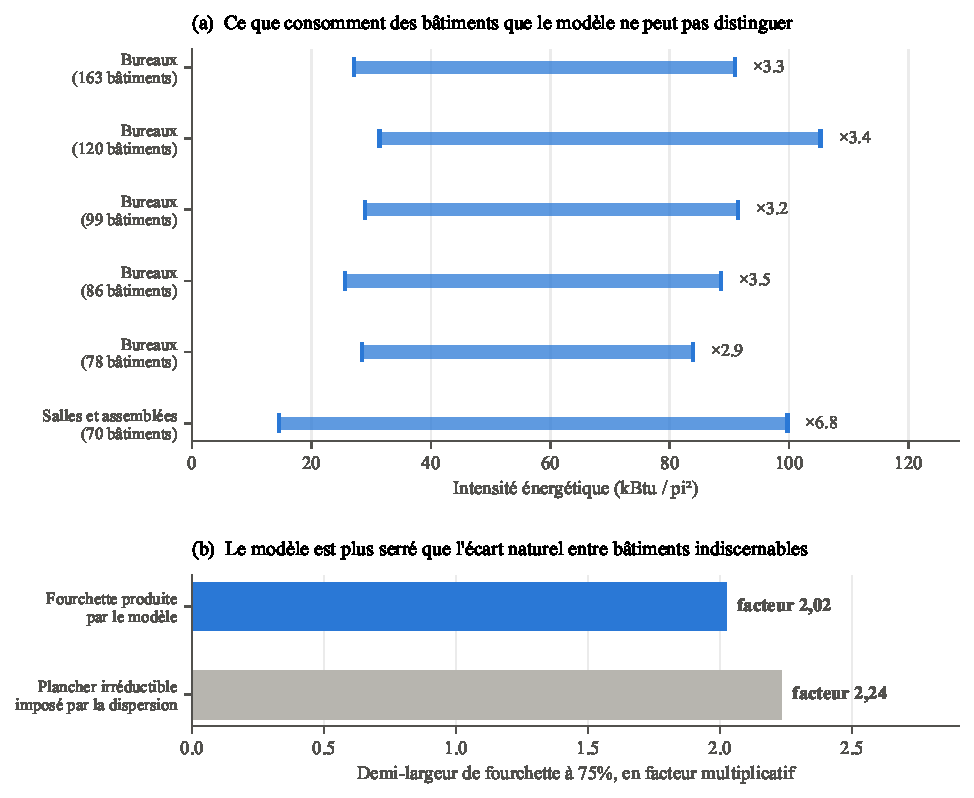
\includegraphics[width=\linewidth]{figures/plafond-performance.pdf}
\caption{En haut, l'étendue réelle des intensités au sein de groupes que le
modèle ne peut pas distinguer. En bas, la conséquence : la dispersion imposerait
à elle seule une fourchette d'un facteur 2,24, alors que le modèle en produit une
de 2,03.}
\end{figure}

\subsubsection*{L'explication physique}

Les variables disponibles décrivent \textbf{ce qu'un bâtiment est}, alors que sa
consommation dépend de \textbf{comment il est utilisé et exploité} :

\begin{itemize}[leftmargin=1.4em,itemsep=0.2em]
  \item le taux d'occupation et les horaires — un plateau à 30\,\% d'occupation
        contre un autre plein, ouvert 40~h ou 90~h par semaine : un facteur~2 à
        lui seul ;
  \item les équipements installés — salle serveurs, cuisine professionnelle,
        imagerie médicale : invisibles dans les données, décisifs dans la facture ;
  \item l'âge et le rendement des systèmes de chauffage et de climatisation ;
  \item la qualité de l'enveloppe — deux immeubles de 1960 dont l'un a été rénové
        sont indiscernables dans ce jeu de données ;
  \item les consignes de température et la régulation.
\end{itemize}

\subsection{Perspectives d'évolution}

\begin{constat}{La marge n'est pas dans l'algorithme}
Six familles de modèles se tiennent en quatre points de $R^2$, et le modèle de
fondation ne gagne que deux points. Investir dans un meilleur algorithme
reviendrait à optimiser la seule dimension qui ne bouge plus.
\end{constat}

Les gains sont dans les \textbf{données}, par ordre décroissant d'effet attendu :

\begin{enumerate}[leftmargin=1.6em,itemsep=0.2em]
  \item données d'occupation — effectifs, horaires d'ouverture ;
  \item inventaire des équipements énergivores ;
  \item âge et type des systèmes de chauffage et de climatisation ;
  \item indicateurs d'enveloppe — année de rénovation, performance thermique ;
  \item sous-comptage par usage.
\end{enumerate}

Deux extensions à moindre coût, indépendantes des données ci-dessus : exploiter
plusieurs millésimes plutôt qu'un seul, ce que le pipeline permet déjà ; et
mesurer l'empreinte de l'inférence, qui n'a pas été instrumentée alors que c'est
elle qui tourne en continu.

\subsection{Prochaines étapes recommandées}

\begin{table}[H]
\centering
\small
\begin{tabularx}{\linewidth}{@{}cXL{2.6cm}@{}}
\toprule
\textbf{Rang} & \textbf{Étape} & \textbf{Effort} \\
\midrule
1 & Confronter la priorisation à des audits réels — c'est le seul moyen de renseigner les indicateurs métier laissés vides & Externe au projet \\
2 & Rejouer le pipeline sur plusieurs millésimes et mesurer la stabilité des estimations dans le temps & Faible \\
3 & Instrumenter l'empreinte de l'inférence et la rapporter au nombre de bâtiments traités & Faible \\
4 & Négocier l'accès à une source d'occupation, même partielle, sur un sous-ensemble du parc & Élevé, hors périmètre technique \\
\bottomrule
\end{tabularx}
\caption{Étapes recommandées, par ordre de valeur.}
\end{table}

\subsection{Limites de la démarche}
\label{sec:limites-demarche}

Trois limites doivent accompagner la lecture de ce rapport.

\begin{description}[leftmargin=0em,style=nextline,itemsep=0.3em]
  \item[Les besoins sont reconstitués.] Aucune partie prenante n'a été
        interrogée. Les besoins ont été déduits de la documentation publique du
        programme et de la nature des données. Une collecte réelle aurait pu
        faire émerger des besoins que ce rapport ignore.
  \item[La garantie de couverture est marginale.] Elle vaut en moyenne sur un
        parc, pas bâtiment par bâtiment, et ne se transporte pas automatiquement
        à chaque typologie. C'est la limite principale de la méthode retenue, et
        elle est écrite dans l'interface.
  \item[Le rendu visuel de l'application n'a pas été vérifié automatiquement.]
        Les tests couvrent le comportement, pas l'apparence ; la vérification
        visuelle est restée manuelle.
\end{description}

\newpage

\section{Annexes}
\markboth{Annexes}{}

\subsection{Liens du projet}

\begin{table}[H]
\centering
\small
\begin{tabularx}{\linewidth}{@{}L{4.2cm}X@{}}
\toprule
\textbf{Livrable} & \textbf{Adresse} \\
\midrule
Application en ligne & \url{https://huggingface.co/spaces/KLEB38/OC_P13_seattle_energy_emission_predictions} \\
Code source & \url{https://github.com/KL38/OC_P13_ML_MLOPS_Building_Energy_model} \\
Données source & \emph{Seattle Building Energy Benchmarking}, millésime 2016, open data municipal \\
\bottomrule
\end{tabularx}
\end{table}

\subsection{Journal des écarts avec la solution auditée}
\label{ann:ecarts}

Chaque ligne a été écrite \emph{au moment} du changement, jamais reconstituée
après coup. C'est cette discipline qui rend la section~2 vérifiable.

\begin{small}
\begin{longtable}{@{}p{0.7cm}p{2.5cm}p{5.2cm}p{5.4cm}@{}}
\toprule
\textbf{Réf.} & \textbf{Étape} & \textbf{Changement} & \textbf{Impact attendu} \\
\midrule
\endfirsthead
\toprule
\textbf{Réf.} & \textbf{Étape} & \textbf{Changement} & \textbf{Impact attendu} \\
\midrule
\endhead
\midrule
\multicolumn{4}{r}{\footnotesize\itshape suite page suivante} \\
\endfoot
\bottomrule
\endlastfoot

E01 & Nettoyage & Deux bâtiments reçoivent leurs propres valeurs d'usage au lieu de celles d'un troisième (copier-coller) & Deux observations fausses en moins \\
E02 & Imputation & Nombre d'étages : 16 valeurs nulles imputées par la médiane calculée (2) au lieu d'une constante codée en dur (4) & Imputation adaptée à une distribution très asymétrique ; se recalcule si les données changent \\
E03 & Nettoyage & Suppression d'une instruction morte (imputation de valeurs manquantes inexistantes) & Aucun sur les valeurs. Lisibilité \\
E04 & Périmètre & Le notebook s'arrête au nettoyage et exporte des données \emph{non transformées} & Permet de rejouer la même préparation à l'entraînement et à l'inférence \\
E05 & Imputation & Nombre de bâtiments : règle conservée, mais justifiée par vérification factuelle plutôt que par proximité à la moyenne & Aucun changement de valeur ; hypothèse défendable en soutenance \\
E06 & Environnement & \code{pandas} épinglé en 2.3.3, non par préférence mais parce que le registre d'expérimentations borne cette dépendance & Aucun sur les valeurs : les notebooks rejoués donnent des résultats identiques \\
E07 & Nettoyage & Quartiers : 19 modalités brutes ramenées à 13 quartiers réels (casse et suffixes) & 29 bâtiments sortis de six catégories fantômes de 1 à 9 individus ; 6 colonnes de moins \\
E08 & \textbf{Fuite de données} & \textbf{Ratios de sources d'énergie remplacés par trois booléens de présence} & \textbf{Écart structurant.} $-10$ points sur les émissions, mais le modèle devient utilisable sur un bâtiment non relevé \\
E09 & Variable & Âge supprimé, année de construction conservée brute & Aucun sur les métriques (transformation affine). Supprime une dérive annuelle mécanique \\
E10 & Composition & Parts d'usage normalisées sur la somme des surfaces déclarées, et non sur la surface totale & La couverture réelle allait de 0 à 6,43 ; la composition devient robuste et correspond à ce que l'interface collecte \\
E11 & Encodage & Quartiers en one-hot (13 colonnes) au lieu d'un encodage binaire (5 colonnes) & Supprime des relations numériques arbitraires entre quartiers et un objet à persister \\
E12 & Variables écartées & Type principal non retenu ; surface totale réduite à son logarithme ; surface bâtie écartée & Évite 21 colonnes redondantes dont plusieurs à moins de 15 exemples \\
E13 & Variable testée & Ratio de parking réintroduit pour contester un arbitrage antérieur, puis retiré après mesure & Aucun écart net au final. \textbf{Un arbitrage de la solution auditée confirmé sur preuve} \\
E14 & Périmètre & Un bâtiment retiré : aucune répartition d'usage déclarée & \num{1655} lignes au lieu de \num{1656}. Point hors domaine qui aurait faussé l'évaluation \\
E15 & Robustesse & Un usage ou un quartier inconnu lève une exception au lieu de produire une colonne fantôme & En production, un bâtiment mal encodé est pire qu'une prédiction refusée \\
E16 & Inférence & L'interface collecte les trois usages principaux \emph{et} le nombre total d'usages déclarés & Supprime un écart entraînement / inférence sur les 9\,\% de bâtiments à plus de trois usages \\
\end{longtable}
\end{small}

\subsubsection*{Écarts assumés, non corrigés}

Relevés pendant le portage, laissés en l'état après décision. Un écart assumé et
documenté vaut mieux qu'un écart oublié.

\begin{table}[H]
\centering
\small
\begin{tabularx}{\linewidth}{@{}L{2.6cm}XL{3.4cm}@{}}
\toprule
\textbf{Étape} & \textbf{Constat} & \textbf{Décision} \\
\midrule
Analyse univariée & Une échelle logarithmique écarte silencieusement les valeurs nulles de trois graphiques : la distribution affichée n'est pas celle des données & Conservé — cosmétique, sans effet sur les données exportées \\
Composition d'usages & Pour les 9\,\% de bâtiments déclarant plus de trois usages, la composition est calculée sur une répartition tronquée puis renormalisée & Conservé — la source ne publie pas mieux, et l'interface applique désormais la même troncature (E16) \\
Général & Commentaires de code en français, contrairement à la convention du projet & Conservé pour garder le portage comparable à la solution auditée \\
\bottomrule
\end{tabularx}
\end{table}


\end{document}
